\documentclass[conference]{IEEEtran}
\IEEEoverridecommandlockouts
% The preceding line is only needed to identify funding in the first footnote. If that is unneeded, please comment it out.
\usepackage{cite}
\usepackage{amsmath,amssymb,amsfonts}
\usepackage{algorithmic}
\usepackage{graphicx}
\usepackage{textcomp}
\usepackage{booktabs}
\usepackage[table,xcdraw]{xcolor}
\usepackage{longtable}
\usepackage{multicol} % Pembuatan kolom ganda
\usepackage{multirow} % Pembuatan baris ganda
\usepackage{xcolor}
\def\BibTeX{{\rm B\kern-.05em{\sc i\kern-.025em b}\kern-.08em
    T\kern-.1667em\lower.7ex\hbox{E}\kern-.125emX}}
\begin{document}

\title{Rekonstruksi Objek Irregular Terpendam pada Beton Berbasis Sinyal Ground-Penetrating Radar Menggunakan Generative Adversarial Network\\
{\footnotesize \textsuperscript{*}Note: Sub-titles are not captured in Xplore and
should not be used}
\thanks{Identify applicable funding agency here. If none, delete this.}
}

\author{\IEEEauthorblockN{1\textsuperscript{st} John Parulian Siahaan}
\IEEEauthorblockA{\textit{Departemen Teknik Komputer} \\
\textit{Fakultas Teknologi Elektro dan Informatika Cerdas}\\
\textit{Institut Teknologi Sepuluh Nopember (ITS)}\\
Surabaya, Indonesia \\
email address or ORCID}
\and
\IEEEauthorblockN{2\textsuperscript{nd} Dion Hayu Fandiantoro, S.T.,M.T.}
\IEEEauthorblockA{\textit{Departemen Teknik Komputer} \\
\textit{Fakultas Teknologi Elektro dan Informatika Cerdas}\\
\textit{Institut Teknologi Sepuluh Nopember (ITS)}\\
City, Country \\
email address or ORCID}
\and
\IEEEauthorblockN{3\textsuperscript{rd} Arief Kurniawan, S.T., M.T.}
\IEEEauthorblockA{\textit{Departemen Teknik Komputer} \\
\textit{Fakultas Teknologi Elektro dan Informatika Cerdas}\\
\textit{Institut Teknologi Sepuluh Nopember (ITS)}\\
City, Country \\
email address or ORCID}
\and
\IEEEauthorblockN{4\textsuperscript{th} Given Name Surname}
\IEEEauthorblockA{\textit{dept. name of organization (of Aff.)} \\
\textit{name of organization (of Aff.)}\\
City, Country \\
email address or ORCID}
\and
\IEEEauthorblockN{5\textsuperscript{th} Given Name Surname}
\IEEEauthorblockA{\textit{dept. name of organization (of Aff.)} \\
\textit{name of organization (of Aff.)}\\
City, Country \\
email address or ORCID}
\and
\IEEEauthorblockN{6\textsuperscript{th} Given Name Surname}
\IEEEauthorblockA{\textit{dept. name of organization (of Aff.)} \\
\textit{name of organization (of Aff.)}\\
City, Country \\
email address or ORCID}
}

\maketitle

\begin{abstract}
\emph{Ground Penetrating Radar} (GPR) sudah sering digunakan dalam ilmu geofisika untuk mendeteksi objek tertimbun bawah tanah. 
Tidak hanya pada media tanah, media lain seperti kayu, beton, dan aspal juga dapat digunakan. 
Objek yang dideteksi juga bisa dalam berbagai bentuk dan materi, salah satunya yaitu \emph{cavities}. 
\emph{Cavities} merupakan rongga udara yang timbul pada beton akibat udara yang terjebak pada proses pengecoran. 
Umumnya bentuk \emph{cavities} adalah irregular. 
Dengan menggunakan sinyal GPR, upaya mendeteksi \emph{cavities} tersebut dapat dilakukan. 
Dalam penelitian ini dilakukan proses rekonstruksi sinyal dari \emph{B-Scan} GPR. 
Bentuk sinyal yang akan digunakan yaitu \emph{ricker wavelet}, karena bentuknya sangat bagus dalam pembentukan data seismik. 
Proses rekonstruksi sinyal umumnya menggunakan transformasi fourier pada saat mengintegrasikan sinyal \emph{A-Scan}, sehingga relatif rumit dan lama. 
Dengan menerapkan \emph{Conditional Generative Adversarial Network} (CGAN), data \emph{B-Scan} GPR dapat disintesis menggunakan fungsi Generator dan Diskriminator. 
Data tersebut dapat digunakan dalam mengidentifikasi dan mengklasifikasi objek pada sinyal GPR, yang fokusan penelitian ini berupa bentuk irregular \emph{cavities} pada beton. 
Dengan penelitian ini, diharapkan terbentuknya suatu metode yang dapat dapat merekonstruksi sinyal \emph{B-Scan} GPR agar lebih sederhana, yang kemudian dapat mendeteksi bentuk irregular \emph{cavities} pada beton.
\end{abstract}

\begin{IEEEkeywords}
Irregular, GPR, B-Scan, CGAN.
\end{IEEEkeywords}

\section{Pendahuluan}
\emph{Ground penetrating radar} (GPR) adalah metode geofisika noninvasif untuk mencitrakan diskontinuitas listrik di bawah permukaan yang dangkal. 
GPR bekerja dengan mengirimkan pulsa elektromagnetik (EM) ke bawah permukaan dan gelombang pantulan direkam oleh antena di permukaan. 
Para peneliti sering menggunakan GPR untuk mempelajari strata bawah permukaan yang dangkal dan untuk mengidentifikasi anomali struktur bawah tanah dalam banyak aplikasi dekat permukaan bumi \cite{a1}. 
\emph{Cavity} merupakan salah satu objek yang dapat diidentifikasi menggunakan GPR.

\emph{Cavity} pada beton merupakan rongga kosong yang terbentuk di dalam maupun di permukaan beton. 
Bentuk \emph{cavities} pada beton biasa tidak beraturan (irregular) karena rongga kecil yang saling bergabung menjadi satu. 
Menurut BPSDM PUPR, kerusakan pada beton akibat rongga udara termasuk dalam kode kerusakan 201 \cite{a2}. 
Kerusakan jenis ini biasa terjadi akibat proses pencampuran yang kurang padat, mengakibatkan beton kehilangan ketahanannya. 
Oleh karena itu, GPR dapat digunakan untuk mengidentifikasi ukuran dan posisi \emph{cavity} pada bawah permukaan beton.

Untuk memperoleh data bentuk struktur geometri bawah permukaan, data mentahan GPR perlu diproses terlebih dahulu. 
Terdapat banyak solusi yang telah dilakukan untuk memproses data GPR, baik metode Numerik seperti \emph{Finite-Difference Time-Domain} (FDTD) \cite{a3}, \emph{Method of Moments} (MoM)\cite{a4}, dan \emph{Finite Element Time-Domain} (FETD)\cite{a5}, 
maupun metode inversi GPR seperti pendekatan \emph{ray-based tomography} \cite{a6}, \emph{reverse-time migration} (RTM), \cite{a7}, dan \emph{full-waveform inversion} (FWI) \cite{a8}.
Namun dari metode tersebut sangat kompleks dalam interpretasinya. 
Interpretasi data GPR, baik metode numerik maupun inversi GPR, relatif rumit karena adanya variasi dalam respons gelombang elektromagnetik yang dihasilkan oleh berbagai struktur dan bahan bawah permukaan. 
Dibutuhkan pengetahuan geologi atau pengalaman yang mendalam dalam interpretasi data untuk menghindari kesalahan atau penafsiran yang salah.

Dalam beberapa tahun terakhir, terdapat metode popular berbasis data seperti \emph{neural networks} dalam aplikasi di banyak bidang ilmiah, dengan keberhasilan yang terkemuka terutama dalam bidang visi komputer dan pemrosesan bahasa natural. 
\emph{Deep neural networks} (DNNs) telah menunjukkan kemampuan luar biasa dalam aplikasi yang berkaitan dengan klasifikasi gambar \cite{a9}, deteksi objek \cite{a10}, dan segmentasi semantik (prediksi tingkat piksel) \cite{a11} dan sintesis gambar \cite{a12}. 
DNN secara otomatis mempelajari fitur tingkat tinggi melalui data pelatihan dan kemudian dapat memperkirakan pemetaan nonlinear antara data gambar masukan dan berbagai domain data, seperti label, teks, atau gambar lainnya. 
Oleh karena itu, beberapa metode inversi berbasis \emph{deep learning end-to-end} telah diperkenalkan untuk membalikkan kecepatan atau impedansi dari data seismik \cite{a13}.

Model generatif adalah bagian dari \emph{neural networks} yang memungkinkan sintesis data yang realistis. 
\emph{Generative Adversarial Networks} (GANs) merupakan bentuk model generatif yang memiliki fungsi Generator untuk menghasilkan suatu data baru melalui pelatihan (\emph{train}) yang dilakukan dan Diskriminator untuk menentukan apakah data baru tersebut merupakan data palsu atau asli. 
Pix2pix merupakan salah satu model GAN yang memiliki kemampuan menerjemahkan \emph{image-to-image}. 
Model ini telah berhasil diterapkan dalam berbagai aplikasi seperti pengolahan citra medis, pemetaan jalan, desain interior, dan seni digital. 
Oleh karena itu, judul ini diajukan dengan harapan model GAN ini dapat merekonstruksi objek irregular terpendam pada beton berbasis sinyal GPR.

Berdasarkan latar belakang tersebut, maka masalah yang dapat diambil adalah proses rekonstruksi sinyal GPR untuk mendeteksi lokasi \emph{cavities} relatif rumit dan lama. 
Terdapat banyak solusi yang telah dilakukan untuk memodelkan objek bawah permukaan, namun metode tersebut membutuhkan proses perhitungan yang rumit dan waktu komputasi yang lama. 
Oleh karena itu, diperlukan suatu metode untuk dapat merekonstruksi objek irregular terpendam pada beton berbasis sinyal GPR.

Tujuan dari penelitian ini adalah membuat suatu metode yang tidak memerlukan proses perhitungan rumit, sehingga dapat merekonstruksi objek irregular terpendam pada beton berbasis sinyal GPR dengan lebih cepat.
Dengan dilaksanakannya penelitian ini, diharapkan terbentuknya suatu metode untuk merekonstruksi objek irregular terpendam pada beton berbasis sinyal GPR yang beresolusi tinggi pada beton dengan menggunakan GAN. 
Selain itu, penelitian ini juga dapat menjadi referensi untuk penelitian selanjutnya terkait rekonstruksi sinyal GPR.

\section{Penelitian Terdahulu}

Dalam pengerjaan penelitian ini, dibutuhkan referensi yang dapat digunakan untuk membantu penelitian. 
Referensi penelitian terkait antara lain penelitian \cite{b1}-\cite{b3}.

Penelitian \cite{b1} merupakan penelitian terkait penerapan metode GAN untuk mendeteksi objek bawah permukaan tanah. 
Dalam penelitiannya, objek yang dideteksi berupa silinder dengan 3 jenis bahan, yaitu besi, plastik, dan beton yang terkubur di bawah permukaan tanah. 
Penelitian ini juga masih menggunakan metode FDTD dalam modelnya. 
Hasil penelitian ini menunjukkan bahwa metode GAN dapat digunakan pada data GPR, baik dari data asli maupun data simulasi GPR. 
Class conditioning dapat diterapkan pada metode GAN dalam menghasilkan training data yang terlabel untuk classifier.

Penelitian \cite{b2} merupakan penelitian yang melakukan 2 metode dalam mendeteksi \emph{cavities} pada beton yang masih baru dicetak, yaitu dengan pendekatan \emph{Infrared Thermographic} dan GPR. 
Penelitian dengan pendekatan GPR bertujuan untuk mengetahui batasan penggunaan GPR pada beton pasca pengecoran. 
Untuk menghindari kerusakan pada beton pasca pengecoran, sebuah papan triplek digunakan sebagai penampang GPR agar tidak menyentuh beton secara langsung. 
Hasil penelitian menunjukkan bahwa GPR dapat menjadi metode \emph{non-destructive testing} (NDT) untuk mendeteksi cavities dengan ukuran 3.8 cm hingga 10 cm pada saat 3 jam setelah pengecoran beton.

Penelitian \cite{b3} merupakan penelitian terkait penggunaan \emph{Conditional Adversial Networks} (CGAN) dalam mengubah dari suatu gambar ke gambar lain. 
Penelitian ini mendemonstrasikan penggunaan pix2pix dalam mensintesis foto dari bentuk label kasaran menjadi suatu gambar objek tertentu. 
Philip Isola beserta timnya menyimpulkan bahwa penggunaan CGAN sangat menjanjikan dalam permasalahan perubahan gambar satu ke gambar lain, terkhususnya yang membutuhkan output terstruktur.

Berdasarkan penelitian referensi tersebut, maka dilakukan penelitian dengan judul Rekonstruksi Objek Irregular Terpendam pada Beton Berbasis Sinyal Ground-Penetrating Radar Menggunakan Generative Adversarial Network”. 
Penelitian ini mengambil ide dari \cite{b1} untuk menggunakan metode GAN dalam mendeteksi objek terpendam bawah permukaan. 
Penelitian ini juga mengambil ide dari \cite{b2} dalam mendeteksi cavities pada bawah permukaan beton menggunakan GPR. 
Penelitian ini juga menggunakan metode \cite{b3} untuk mengubah dari gambar B-scan menjadi gambar prediksi bentuk dan posisi objek pada bawah permukaan beton.

\section{Uraian Penelitian}
Penelitian ini dilaksanakan sesuai dengan metodologi yang telah dirancang. 
Metodologi terbagi menjadi 4 tahap, yaitu pengumpulan data, pembentukan arsitektur GAN, training model, dan evaluasi model. 
Gambar \ref{fig:metodologi} menunjukkan diagram dari metodologi penelitian.

\begin{figure}[ht]
  \centering
  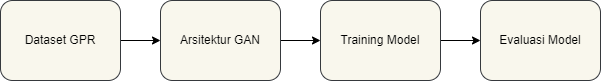
\includegraphics[scale=0.35]{gambar/metodologi.png}
  \caption{Diagram Metodologi Penelitian}
  \label{fig:metodologi}
\end{figure}

\subsection{Dataset GPR}\label{DatasetGPR}
Tahap ini merupakan tahap pengumpulan dataset GPR. 
Data yang dibutuhkan ada 2 jenis, yaitu data input berupa gambar B-scan GPR hasil simulasi gprMax dan data output yang diharapkan berupa gambar bentuk geometri dari gambar B-scan GPR. 
Alur dari proses pengumpulan dataset ditampilkan pada gambar \ref{fig:datasetgpr}.

\begin{figure}[ht]
  \centering
  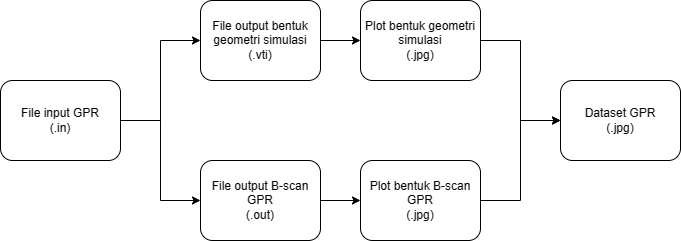
\includegraphics[scale=0.35]{gambar/alur pengumpulan data.png}
  \caption{Diagram Pengumpulan Dataset GPR}
  \label{fig:datasetgpr}
\end{figure}

Simulasi menggunakan gprMax untuk menghasilkan file output bentuk geometri simulasi dan file output B-scan GPR dengan menggunakan file input gprMax. 
Setiap kebutuhan dan cara instalasi gprMax dapat diperoleh di github gprMax. 
Dalam memasang gprMax, dibutuhkan untuk memasang Python, Miniconda/Anaconda, dan C Compiler yang mendukung OpenMP (Desktop development with C++ pada Visual Studio untuk OS Windows). \\

Dalam menyusun kode program input GPR, dibutuhkan beberapa parameter penyusun yang perlu diperhatikan. 
Parameter penyusun tersebut dapat dilihat pada panduan gprMax di website resmi gprMax. 
Pada penelitian ini, parameter sistem yang dibuat pada dataset GPR dapat dilihat pada tabel \ref{tb:inputGPR}. 
Contoh penggunaan parameter pada file input juga dapat dilihat pada gambar \ref{fig:inputgprMax}.

\begin{table}[htbp]
    \caption{Parameter Input GprMax}
    \begin{center}
    \begin{tabular}{|c|c|c|}
    \hline
    \textbf{Parameter} & \textbf{Nilai} \\
    \hline
    Dimensi                     & 0.3 m x 0.3 m x 0.001 m                   \\
    Jendela Waktu               & 3 ns                                      \\
    Material                    & Beton (medium) dan ruang kosong (objek)   \\
    Basis Sinyal                & Ricker                                    \\
    Arah Laju Sumber Sinyal     & 0.001 m/step terhadap sumbu-X             \\
    Bentuk Objek                & Tabung                                    \\
    \hline
    \end{tabular}
    \label{tb:inputGPR}
    \end{center}
\end{table}

\begin{figure}[ht]
  \centering
  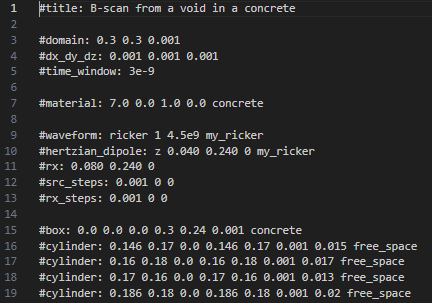
\includegraphics[scale=0.6]{gambar/inputGprMax.png}
  \caption{Contoh isi file input gprMax}
  \label{fig:inputgprMax}
\end{figure}

Data input gprMax di atas kemudian disimulasikan dengan 2 tools berbeda untuk menghasilkan file output bentuk geometri simulasi dan file output B-scan GPR. 
Dari proses simulasi, diperoleh dua buah hasil, yaitu file output bentuk geometri simulasi (.vti) dan file output B-scan GPR (.out). 
Untuk memperoleh gambar bentuk geometri simulasi, file output bentuk geometri simulasi dijalankan menggunakan aplikasi Paraview. 
Sedangkan untuk memperoleh gambar bentuk sinyal B-scan GPR, file output B-scan GPR dijalankan menggunakan tools dari gprMax.

Kedua jenis gambar ini kemudian digabung menjadi satu gambar dengan menggunakan library PIL. 
Kedua gambar akan disusun horizontal, dimana gambar yang kiri berupa gambar B-scan gprMax dan gambar yang kanan berupa gambar bentuk geometrinya. 
Contoh gabungan gambar ditampilkan pada gambar \ref{fig:contohdata}. 
Gambar hasil gabungan ini yang kemudian menjadi dataset model GAN yang akan dibentuk, yang dalam penelitian ini menggunakan sejumlah 200 data.

\begin{figure}[ht]
  \centering
  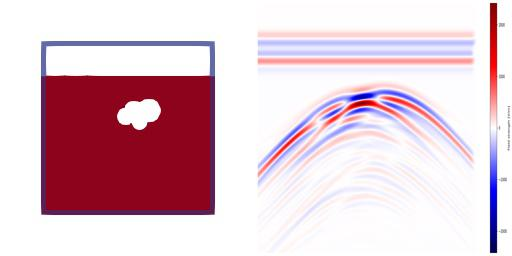
\includegraphics[scale=0.5]{gambar/data1.jpg}
  \caption{Gambar gabungan bentuk geometri bawah permukaan (kiri) dengan bentuk B-scan GPR hasil simulasi (kanan)}
  \label{fig:contohdata}
\end{figure}

\subsection{Arsitektur GAN}
Setelah dataset berhasil dikumpulkan, selanjutnya akan dibentuk model dari GAN. 
Model GAN yang akan dibentuk menggunakan model Conditional GAN Pix2pix. 
Arsitektur GAN akan dibagi menjadi 2 bagian, yaitu bagian generator yang berfungsi untuk mensintesis gambar seperti data asli, dan bagian diskriminator yang berfungsi untuk membedakan antara data asli dengan data hasil sintesis. 
Bentuk arsitektur GAN ditampilkan pada gambar \ref{fig:arsitekturGAN}.

\begin{figure}[ht]
  \centering
  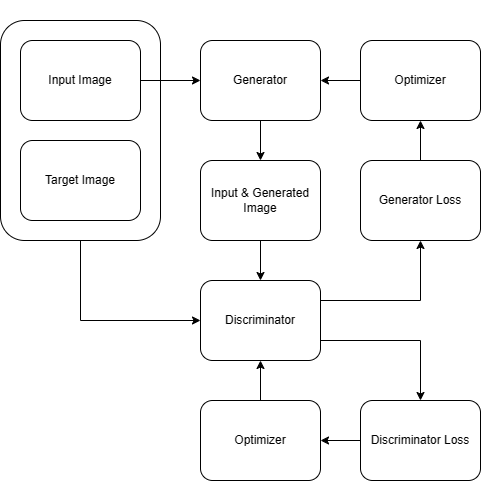
\includegraphics[scale=0.45]{gambar/Arsitektur GAN.png}
  \caption{Diagram Arsitektur GAN yang Dibentuk}
  \label{fig:arsitekturGAN}
\end{figure}

\newpage

Pada bagian generator, digunakan arsitektur U-net \cite{c1}. 
Arsitektur ini terdiri dari jaringan encoder yang dilanjut dengan jaringan decoder. 
Jaringan encoder akan menerapkan proses Convolution $>>$ Batch normalization $>>$ Leaky ReLU. 
Sedangkan decoder akan menerapkan proses Transposed convolution $>>$ Batch normalization $>>$ Dropout (untuk 3 blok pertama) $>>$ ReLU. 
Tiap pasang encoder-decoder memiliki skip connection yang berfungsi untuk menangkap setiap informasi tingkat rendah yang dibagikan antara input dan output. 
Diagram arsitektur Generator dapat dilihat pada gambar \ref{fig:generator}.

\begin{figure}[ht]
  \centering
  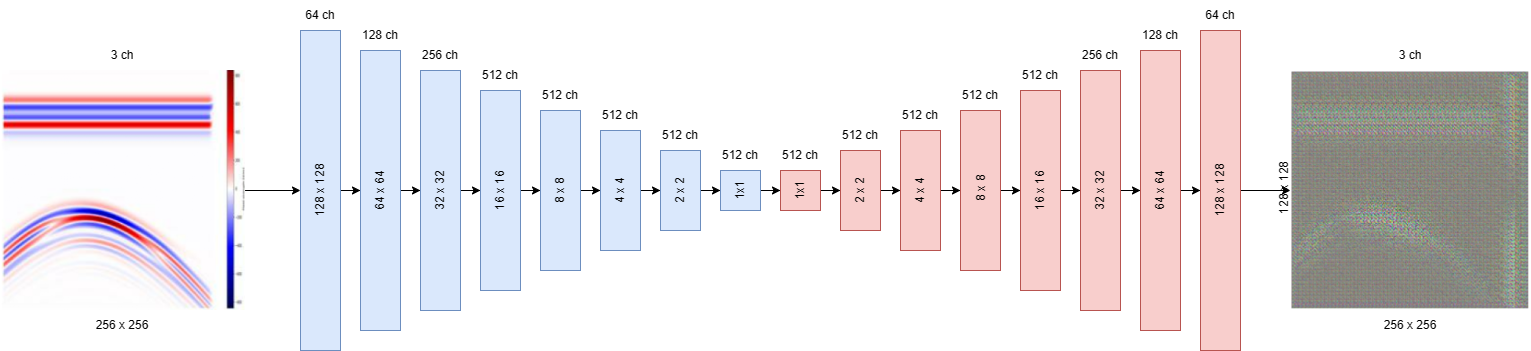
\includegraphics[scale=0.15]{gambar/Generator.png}
  \caption{Diagram Arsitektur Generator}
  \label{fig:generator}
\end{figure}

Pada bagian discriminator, digunakan arsitektur Convolutional Patch GAN yang akan mencoba mengklasifikasikan sepetak (30 x 30) gambar itu nyata atau tidak. 
Discriminator akan menerima dua pasang gambar sebagai input, yaitu gambar input-asli dan gambar input-sintesis. 
Masing-masing pasangan input ini akan digabung terlebih dahulu sebelum masuk ke jaringan encoder. 
Diagram arsitektur Discriminator dapat dilihat pada gambar \ref{fig:discriminator}.

\begin{figure}[ht]
  \centering
  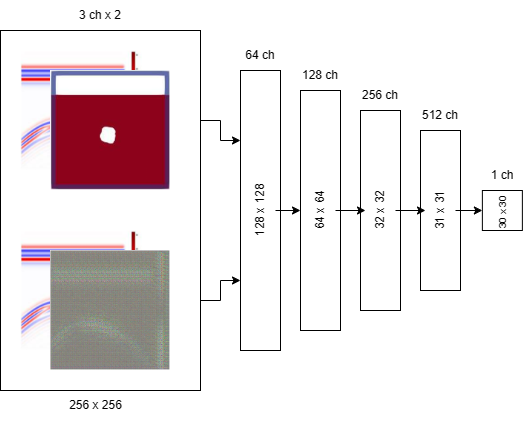
\includegraphics[scale=0.3]{gambar/Discriminator.png}
  \caption{Diagram Arsitektur Discriminator}
  \label{fig:discriminator}
\end{figure}

Generator Loss merupakan gabungan dari sigmoid cross-entropy loss antara gambar yang dihasilkan dengan suatu array 1 (GAN Adversial Loss), dan MAE (Mean Absolute Error) antara gambar yang disintesis dengan gambar asli(L1 Loss). 
Secara matematis, nilai dari Total Generator Loss dapat didefinisikan sebagai 

\begin{equation}
  \label{eq:genLoss}
  Total Gen Loss = GAN Adversial Loss + (\lambda * L_{1} Loss) 
\end{equation}

dimana $\lambda$ dapat didefisinikan sesuai keinginan model (pada penelitian ini $\lambda$ = 100).

Discriminator Loss terdiri dari sigmoid cross-entropy loss antara gambar asli dengan array 1 (Real Loss), dan sigmoid cross-entropy loss antara gambar yang dihasilkan dengan array 0 (Generated Loss). 
Total Discriminator Loss merupakan jumlah dari Real Loss dan Generated Loss

Pada model GAN juga didefinisikan fungsi optimizer dan checkpoint.
Fungsi optimizer menggunakan Adaptive Moment Estimation (Adam) baik untuk generator maupun diskriminator. 
Fungsi checkpoint digunakan untuk menyimpan hasil sementara (checkpoint) dari hasil pelatihan generator dan diskriminator model GAN.

\subsection{Training Model}
Arsitektur GAN yang telah dibentuk kemudian diteruskan ke proses training. 
Alur keseluruhan Training Model dapat dilihat pada gambar \ref{fig:training}. 
Dari 200 data pada dataset, 160 digunakan untuk proses training model. 
Proses training model ini dilakukan sebanyak 40000 iterasi. 
Untuk setiap 1000 iterasi, akan ditampilkan proses sintesis gambar, dan untuk setiap 5000 iterasi, checkpoint dari model akan disimpan.

\begin{figure}[ht]
  \centering
  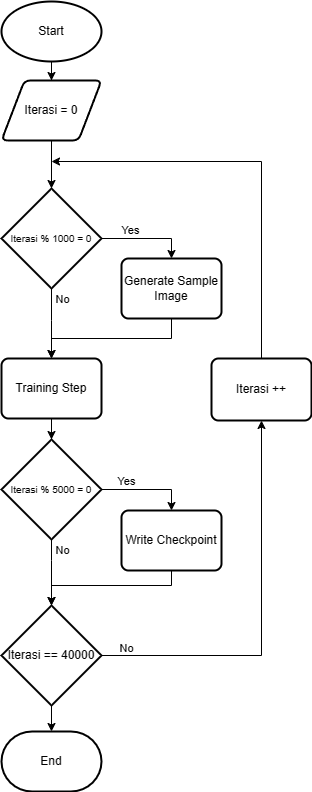
\includegraphics[scale=0.5]{gambar/Training_model.png}
  \caption{Diagram Proses Training Model Keseluruhan}
  \label{fig:training}
\end{figure}

Untuk setiap 1 iterasi proses training, model akan menjalankan proses yang alurnya dapat dilihat pada gambar \ref{fig:arsitekturGAN}. 
Gambar Input akan dimasukkan ke Generator, dan akan menghasilkan Gambar sintesis. 
Discriminator akan memproses 2 pasangan input, yaitu pasangan gambar input dengan gambar asli, dan pasangan gambar input dengan gambar sintesis. 
Pada pasangan pertama, akan diperoleh output Discriminator dari gambar asli, dan pasangan kedua akan diperoleh output Discriminator dari gambar sintesis. 

Generator Loss akan memproses output Discriminator dari gambar sintesis, bersama dengan gambar hasil sintesis dan gambar asli. 
Hasil dari Total Generator Loss akan diterima oleh Generator Optimizer, dan akan diterapkan ke Generator di iterasi berikutnya. 
Discriminator Loss akan memproses output Discriminator dari gambar sintesis dan dari gambar asli. 
Hasil dari Total Discriminator Loss akan diterima oleh Discriminator Optimizer, dan akan diterapkan ke Discriminator di iterasi berikutnya.

\subsection{Evaluasi Model}
Setelah model mengalami proses training, model akan dites dengan menggunakan test data. 
Test data berupa 40 data dari dataset yang belum dilatih pada model. 
\emph{Checkpoint} yang disimpan terakhir akan dimuat, dan akan dicoba untuk mensintesis gambar menggunakan test data tersebut. 

Proses evaluasi dilakukan dengan evaluasi matriks kemudian dilanjut dengan evaluasi visual. 
Evaluasi matriks adalah metode objektif yang menggunakan berbagai metrik dan parameter numerik untuk mengukur sejauh mana dua gambar cocok atau berbeda. 
Metode evaluasi matriks yang digunakan pada penelitian ini adalah metode \emph{Root Mean Square} (RMS), \emph{Mean Square Error} (MSE) dan \emph{Structural Similarity Index} (SSIM). 
RMS dan MSE umumnya digunakan untuk mengukur kesalahan atau perbedaan antara dua gambar atau sinyal, dengan nilai yang lebih rendah menunjukkan kesamaan yang lebih besar. 
Sedangkan SSIM memberikan ukuran yang lebih holistik tentang kesamaan struktural antara dua gambar.

Setelah melakukan evaluasi matriks, dilakukan evaluasi visual. 
Evaluasi visual dilakukan dengan melibatkan penilaian subjektif oleh manusia terhadap kualitas dan kemiripan dua gambar. 
Dalam membantu proses evaluasi visual, digunakan fungsi \emph{image differencing}. 
Fungsi \emph{image differencing} melibatkan pengurangan piksel-piksel dari gambar asli dengan gambar sintesis. 
Hasil pengurangan dapat mengungkapkan informasi penting tentang perubahan struktur, pergeseran objek, atau perubahan lainnya dalam gambar.

\section*{Hasil dan Diskusi}

\subsection{Dataset GPR}
Penelitian ini menggunakan dataset GPR buatan sendiri dari hasil simulasi gprMax. 
Simulasi gprMax dilakukan untuk mendapat 2 jenis data, yaitu data gambar \emph{B-scan} GPR dan data gambar bentuk geometri simulasi. 
Untuk data gambar \emph{B-scan} membutuhkan waktu sekitar 15-20 menit per simulasi, sedangkan untuk data gambar bentuk geometri simulasi membutuhkan waktu sekitar 5-10 menit per simulasi. 
Sehingga total waktu yang dibutuhkan untuk mensimulasikan 200 dari data gambar \emph{B-scan} GPR dan data gambar bentuk geometri simulasi serta penggabungan kedua data menjadi satu sekitar 85 jam.

Dari 200 data GPR, 160 data digunakan untuk proses pelatihan model dan 40 data untuk proses evaluasi model. 
Parameter simulasi pada data ini dibuat acak dengan batasan tertentu untuk data pelatihan dan dibuat menyesuaikan variasi untuk data test. 
Dataset penelitian divariasikan berdasarkan kategori sebagai berikut.

\begin{enumerate}[nolistsep]

  \item Objek berbentuk regular

  \item Kompleksitas bentuk objek

  \item Ukuran objek
  
  \item Posisi objek di bawah permukaan

\end{enumerate}

Pada kategori variasi objek berbentuk regular, data dibedakan berdasar bentuk reguler objek, yaitu data dengan objek berbentuk lingkaran (silinder tampak depan) dan data dengan objek berbentuk segi empat (silinder tampak samping). 
Objek hanya terdiri dari 1 objek penyusun, dengan posisi dan ukuran yang dibebaskan, yaitu posisi sekitar 2.5-10 cm di bawah permukaan dan ukuran sekitar 3-10 cm. 
Contoh data untuk variasi ini dapat dilihat pada gambar \ref{fig:regularData}.

\begin{figure}[ht]
  \centering
  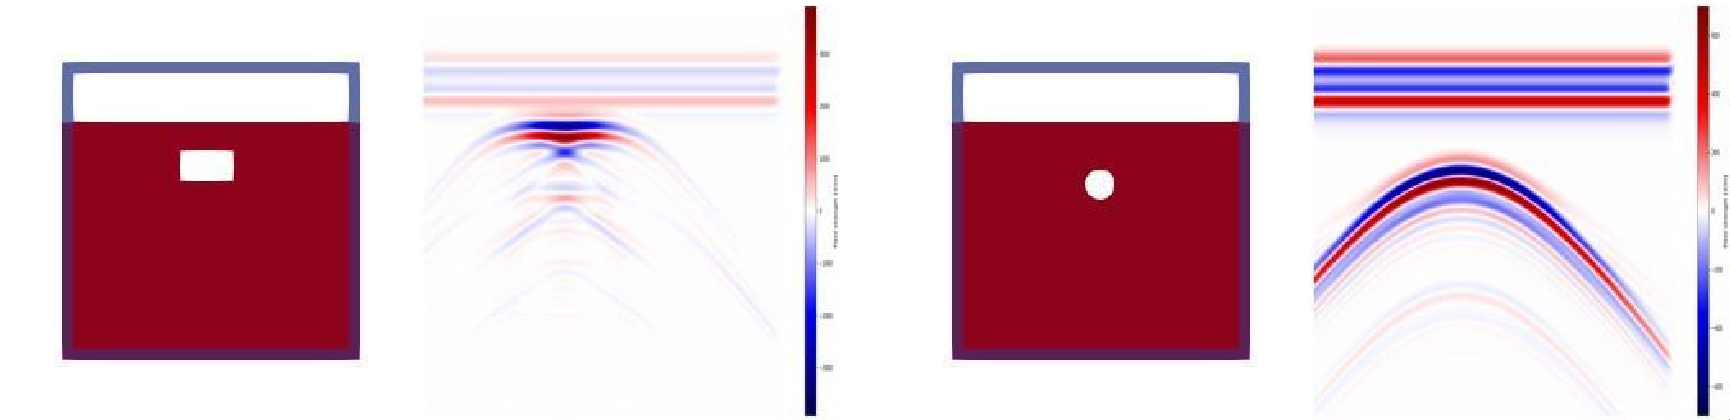
\includegraphics[scale=0.2]{gambar/variasi reguler.png}
  \caption{Data dengan Objek Berbentuk Lingkaran (Kanan) dan Data dengan Objek Berbentuk Segi Empat (Kiri)}
  \label{fig:regularData}
\end{figure}

Pada kategori variasi kompleksitas bentuk objek, data dibedakan berdasar banyak objek penyusun yang digabung, yaitu data dengan objek sederhana dan data dengan objek kompleks. 
Objek sederhana memiliki sekitar 3-6 objek penyusun, sedangkan objek kompleks memiliki sekitar 10-15 objek penyusun. 
Posisi objek dan ukuran objek penyusun kedua data disamakan, yaitu posisi sekitar 6.5 cm di bawah permukaan dan ukuran objek penyusun sekitar 1.5 cm. 
Contoh data untuk variasi ini dapat dilihat pada gambar \ref{fig:kompleksData}.

\begin{figure}[ht]
  \centering
  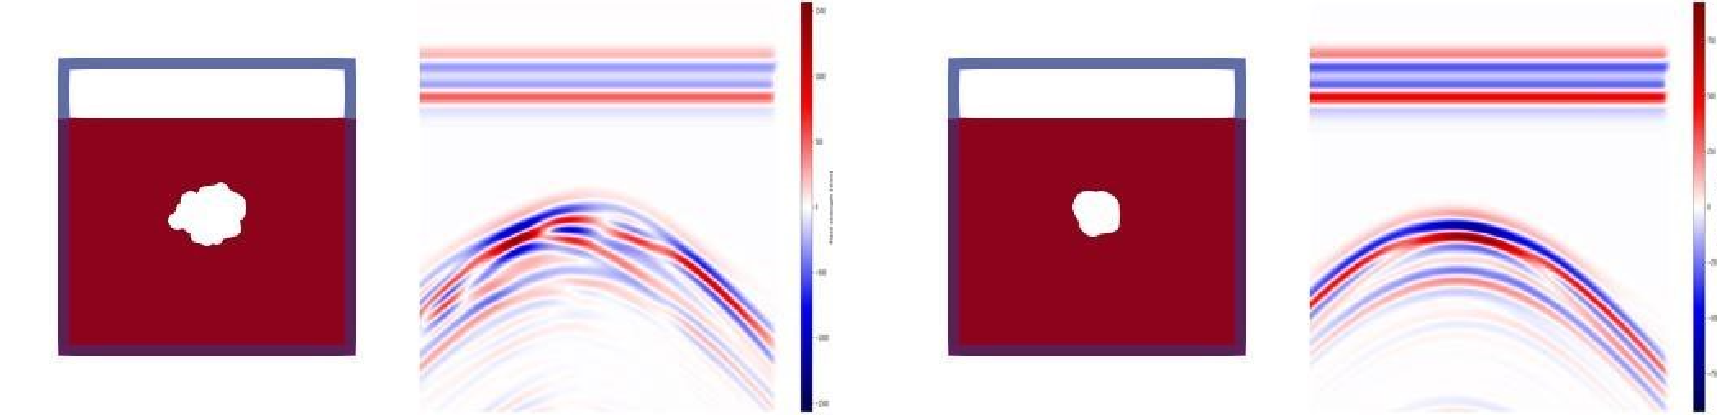
\includegraphics[scale=0.2]{gambar/variasi kompleksitas.png}
  \caption{Data dengan Objek Berbentuk Sederhana (Kanan) dan Data dengan Objek Berbentuk Kompleks (Kiri)}
  \label{fig:kompleksData}
\end{figure}

Pada kategori variasi ukuran objek, data dibedakan berdasar besar ukuran objek, yaitu data dengan objek kecil dan data dengan objek besar. 
Objek kecil memiliki ukuran sekitar 3-4 cm, sedangkan objek besar memiliki ukuran sekitar 5-6 cm. 
Jumlah objek penyusun serta posisi objek disamakan, yaitu objek penyusun sejumlah 5 buah dan kedalaman sekitar 4.5 cm. 
Contoh data untuk variasi ini dapat dilihat pada gambar \ref{fig:ukuranData}.

\begin{figure}[ht]
  \centering
  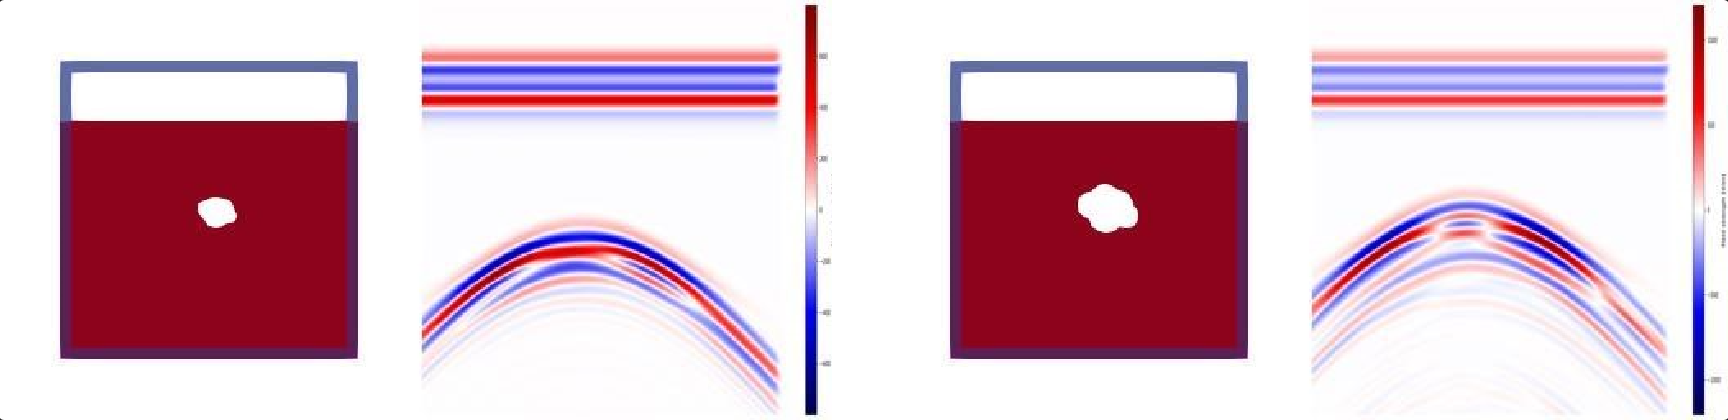
\includegraphics[scale=0.2]{gambar/variasi ukuran.png}
  \caption{Data dengan Objek Berukuran Besar (Kanan) dan Data dengan Objek Berukuran Kecil (Kiri)}
  \label{fig:ukuranData}
\end{figure}

Pada kategori variasi Posisi objek di bawah permukaan, data dibedakan berdasar posisi objek dari permukaan, yaitu data dengan objek dangkal dan data dengan objek dalam. 
Objek dangkal memiliki posisi sekitar 2.5 cm dari permukaan, sedangkan objek dalam memiliki posisi sekitar 7.5 cm dari permukaan. 
Ukuran objek dan jumlah objek penyusun disamakan, yaitu ukuran objek sekitar 4.5 cm dan jumlah objek penyusun sejumlah 5 buah. 
Contoh data untuk variasi ini dapat dilihat pada gambar \ref{fig:posisiData}.

\begin{figure}[ht]
  \centering
  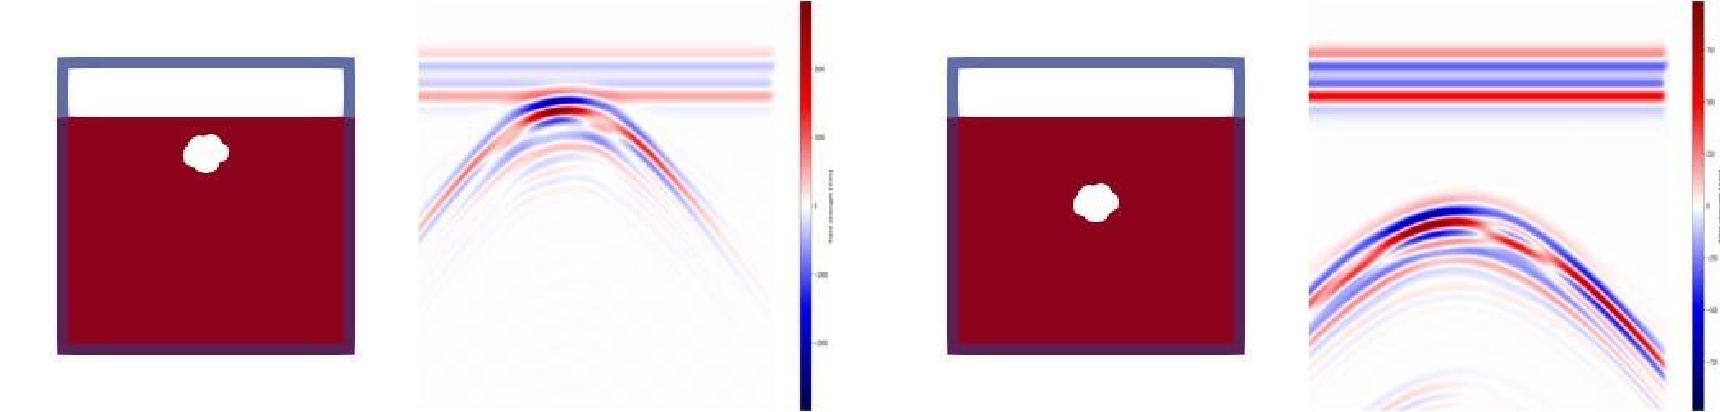
\includegraphics[scale=0.2]{gambar/variasi kedalaman.png}
  \caption{Data dengan Posisi Objek Jauh dari Permukaan (Kanan) dan Data dengan Posisi Objek Dekat dari Permukaan (Kiri)}
  \label{fig:posisiData}
\end{figure}

\subsection{Hasil Pelatihan Model GAN}

Proses pelatihan model dilakukan sebanyak 40.000 iterasi. 
Total waktu yang diperlukan untuk menjalankan keseluruhan proses pelatihan selama 9 jam mulai jam 20.00 WIB hingga pukul 05.00 WIB esok harinya. 
Selama pelatihan, nilai \emph{total discriminator loss} dan \emph{total generator loss} disimpan ke sebuah \emph{log}. 
Dengan menggunakan tensorboard, nilai \emph{loss} yang disimpan pada \emph{log} dapat divisualisasikan dalam bentuk grafik. 

\begin{figure}[ht]
  \centering
  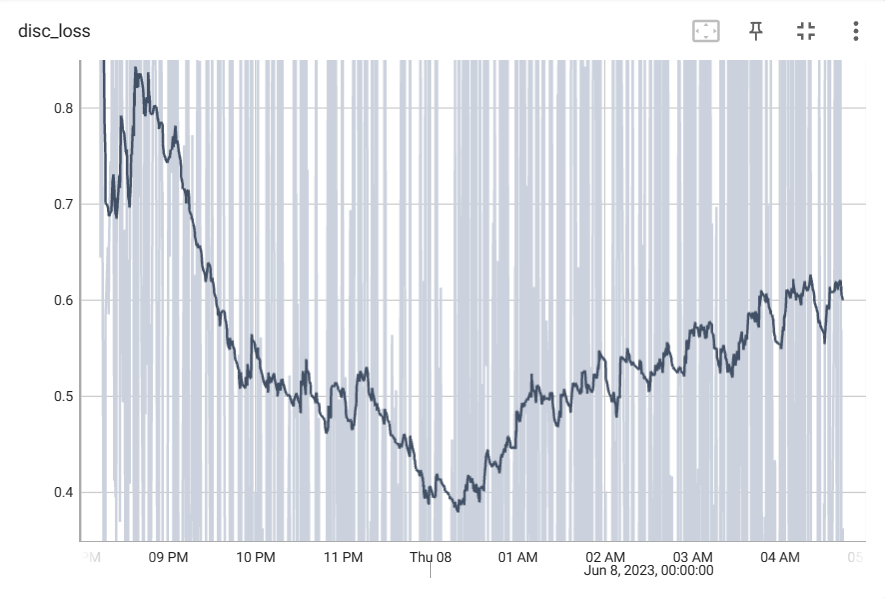
\includegraphics[scale=0.4]{gambar/Disc_loss.png}
  \caption{Grafik Total Discriminator Loss}
  \label{fig:discLoss}
\end{figure}

Gambar \ref{fig:discLoss} menunjukkan grafik \emph{discriminator loss} yang awalnya semakin mengecil kemudian mengalami peningkatan. 
Hal ini menunjukkan bahwa discriminator awalnya semakin baik dalam mempelajari perbedaan data asli dengan data yang disintesis. 
Setelah melewati waktu tertentu, discriminator kemudian menjadi semakin sulit dalam mempelajari perbedaan tersebut. 

\begin{figure}[ht]
  \centering
  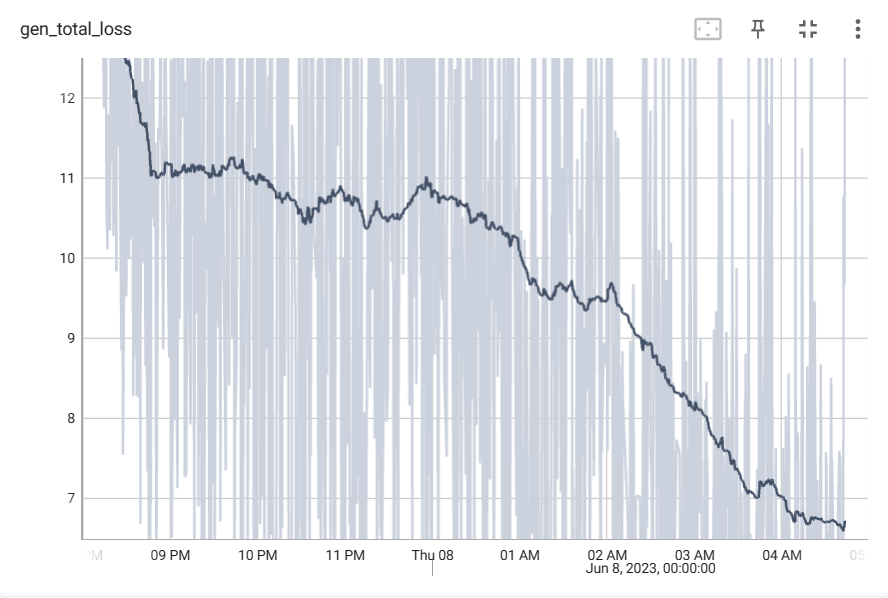
\includegraphics[scale=0.4]{gambar/Gen_total_loss.png}
  \caption{Grafik Total Generator Loss}
  \label{fig:genLoss}
\end{figure}

Gambar \ref{fig:genLoss} menunjukkan grafik \emph{generator loss} yang semakin lama semakin mengecil. 
Hal ini menunjukkan bahwa generator semakin baik dalam mempelajari dan menghasilkan data sintesis yang sesuai dengan data asli. 
Grafik juga menunjukkan penurunan nilai yang lumayan konstan, sehingga dapat dikatakan model generator dilatih secara baik pada proses pelatihan model GAN.

Dalam proses pelatihan model GAN, penting untuk membandingkan nilai atau grafik \emph{generator loss} dan \emph{discriminator loss}. 
Pada kedua grafik, dapat dilihat bahwa awalnya perubahan kedua nilai \emph{loss} sama-sama menurun, yang menunjukkan proses model dalam mempelajari data berjalan dengan baik. 
Namun, sekitar pukul 00.00 grafik dari \emph{discriminator loss} menjadi semakin meningkat, sedangkan grafik \emph{generator loss} tetap semakin menurun. 
Hal ini menunjukkan bahwa pada interval waktu tersebut, discriminator sudah mulai kesulitan dalam membedakan gambar asli dengan gambar palsu, sedangkan generator tetap semakin baik dalam menghasilkan output yang sesuai dengan aslinya.

\subsection{Hasil Evaluasi Output GAN}

Data penelitian menggunakan 200 data hasil simulasi gprMax untuk gambar \emph{B-scan} GPR beserta bentuk geometri dari simulasi. 
Dari 200 total data, 40 data digunakan sebagai test data dan dilakukan evaluasi model GAN. 
Proses evaluasi dilakukan dengan evaluasi matriks kemudian dilanjut dengan evaluasi visual. 
Evaluasi matriks dilakukan dengan menggunakan 3 metode, yaitu metode RMS, MSE, dan SSIM. 
Untuk nilai hasil RMS dan MSE dikatakan baik jika nilainya semakin mendekati 0, sedangkan untuk nilai hasil SSIM dikatakan baik jika nilainya semakin mendekati 1. 
Hasil dari evaluasi matriks untuk keseluruhan data dapat dilihat pada tabel \ref{tb:evaluasimatriks}. 

\begin{table}[]
  \caption{Tabel Nilai RMS, MSE dan SSIM dari Gambar Sintesis dengan Gambar Asli Setiap Variasi Data}
  \label{tb:evaluasimatriks}
  \begin{tabular}{|l|cc|cc|cc|}
  \hline
  \multicolumn{1}{|c|}{Variasi Data}                  & \multicolumn{2}{c|}{RMS}                                                                               & \multicolumn{2}{c|}{MSE}                                                                                   & \multicolumn{2}{c|}{SSIM}                                                                            \\ \hline
                                                      & \multicolumn{1}{c|}{\cellcolor[HTML]{FFFFFF}24.34} & \cellcolor[HTML]{FFFFFF}                         & \multicolumn{1}{c|}{\cellcolor[HTML]{FFFFFF}849.06}  & \cellcolor[HTML]{FFFFFF}                           & \multicolumn{1}{c|}{\cellcolor[HTML]{FFFFFF}0.86} & \cellcolor[HTML]{FFFFFF}                        \\ \cline{2-2} \cline{4-4} \cline{6-6}
                                                      & \multicolumn{1}{c|}{\cellcolor[HTML]{FFFFFF}23.52} & \cellcolor[HTML]{FFFFFF}                         & \multicolumn{1}{c|}{\cellcolor[HTML]{FFFFFF}925.55}  & \cellcolor[HTML]{FFFFFF}                           & \multicolumn{1}{c|}{\cellcolor[HTML]{FFFFFF}0.85} & \cellcolor[HTML]{FFFFFF}                        \\ \cline{2-2} \cline{4-4} \cline{6-6}
                                                      & \multicolumn{1}{c|}{\cellcolor[HTML]{FFFFFF}26.17} & \cellcolor[HTML]{FFFFFF}                         & \multicolumn{1}{c|}{\cellcolor[HTML]{FFFFFF}1232.39} & \cellcolor[HTML]{FFFFFF}                           & \multicolumn{1}{c|}{\cellcolor[HTML]{FFFFFF}0.83} & \cellcolor[HTML]{FFFFFF}                        \\ \cline{2-2} \cline{4-4} \cline{6-6}
                                                      & \multicolumn{1}{c|}{\cellcolor[HTML]{FFFFFF}24.36} & \cellcolor[HTML]{FFFFFF}                         & \multicolumn{1}{c|}{\cellcolor[HTML]{FFFFFF}1047.61} & \cellcolor[HTML]{FFFFFF}                           & \multicolumn{1}{c|}{\cellcolor[HTML]{FFFFFF}0.84} & \cellcolor[HTML]{FFFFFF}                        \\ \cline{2-2} \cline{4-4} \cline{6-6}
  \multirow{-5}{*}{Lingkaran}          & \multicolumn{1}{c|}{\cellcolor[HTML]{FFFFFF}24.05} & \multirow{-5}{*}{\cellcolor[HTML]{FFFFFF}24.487} & \multicolumn{1}{c|}{\cellcolor[HTML]{FFFFFF}1056.576} & \multirow{-5}{*}{\cellcolor[HTML]{FFFFFF}1022.24} & \multicolumn{1}{c|}{\cellcolor[HTML]{FFFFFF}0.84} & \multirow{-5}{*}{\cellcolor[HTML]{FFFFFF}0.84} \\ \hline
                                                      & \multicolumn{1}{c|}{26.549}                         & \cellcolor[HTML]{FFFFFF}                         & \multicolumn{1}{c|}{1160.14}                         & \cellcolor[HTML]{FFFFFF}                           & \multicolumn{1}{c|}{0.84}                         & \cellcolor[HTML]{FFFFFF}                        \\ \cline{2-2} \cline{4-4} \cline{6-6}
                                                      & \multicolumn{1}{l|}{28.027}                         & \cellcolor[HTML]{FFFFFF}                         & \multicolumn{1}{l|}{1060.92}                         & \cellcolor[HTML]{FFFFFF}                           & \multicolumn{1}{l|}{0.85}                         & \cellcolor[HTML]{FFFFFF}                        \\ \cline{2-2} \cline{4-4} \cline{6-6}
                                                      & \multicolumn{1}{l|}{24.116}                         & \cellcolor[HTML]{FFFFFF}                         & \multicolumn{1}{l|}{919.71}                          & \cellcolor[HTML]{FFFFFF}                           & \multicolumn{1}{l|}{0.86}                         & \cellcolor[HTML]{FFFFFF}                        \\ \cline{2-2} \cline{4-4} \cline{6-6}
                                                      & \multicolumn{1}{l|}{27.656}                         & \cellcolor[HTML]{FFFFFF}                         & \multicolumn{1}{l|}{1266.81}                         & \cellcolor[HTML]{FFFFFF}                           & \multicolumn{1}{l|}{0.83}                         & \cellcolor[HTML]{FFFFFF}                        \\ \cline{2-2} \cline{4-4} \cline{6-6}
  \multirow{-5}{*}{Segi Empat}         & \multicolumn{1}{l|}{30.18}                         & \multirow{-5}{*}{\cellcolor[HTML]{FFFFFF}27.305} & \multicolumn{1}{l|}{1395.07}                         & \multirow{-5}{*}{\cellcolor[HTML]{FFFFFF}1160.53} & \multicolumn{1}{l|}{0.81}                         & \multirow{-5}{*}{\cellcolor[HTML]{FFFFFF}0.84} \\ \hline
                                                      & \multicolumn{1}{c|}{\cellcolor[HTML]{FFFFFF}28.45} & \cellcolor[HTML]{FFFFFF}                         & \multicolumn{1}{c|}{\cellcolor[HTML]{FFFFFF}1416.19} & \cellcolor[HTML]{FFFFFF}                           & \multicolumn{1}{c|}{\cellcolor[HTML]{FFFFFF}0.85} & \cellcolor[HTML]{FFFFFF}                        \\ \cline{2-2} \cline{4-4} \cline{6-6}
                                                      & \multicolumn{1}{c|}{\cellcolor[HTML]{FFFFFF}30.69} & \cellcolor[HTML]{FFFFFF}                         & \multicolumn{1}{c|}{\cellcolor[HTML]{FFFFFF}1753.31} & \cellcolor[HTML]{FFFFFF}                           & \multicolumn{1}{c|}{\cellcolor[HTML]{FFFFFF}0.81} & \cellcolor[HTML]{FFFFFF}                        \\ \cline{2-2} \cline{4-4} \cline{6-6}
                                                      & \multicolumn{1}{c|}{\cellcolor[HTML]{FFFFFF}29.96} & \cellcolor[HTML]{FFFFFF}                         & \multicolumn{1}{c|}{\cellcolor[HTML]{FFFFFF}1658.96} & \cellcolor[HTML]{FFFFFF}                           & \multicolumn{1}{c|}{\cellcolor[HTML]{FFFFFF}0.83} & \cellcolor[HTML]{FFFFFF}                        \\ \cline{2-2} \cline{4-4} \cline{6-6}
                                                      & \multicolumn{1}{c|}{\cellcolor[HTML]{FFFFFF}25.72} & \cellcolor[HTML]{FFFFFF}                         & \multicolumn{1}{c|}{\cellcolor[HTML]{FFFFFF}1341.36} & \cellcolor[HTML]{FFFFFF}                           & \multicolumn{1}{c|}{\cellcolor[HTML]{FFFFFF}0.84} & \cellcolor[HTML]{FFFFFF}                        \\ \cline{2-2} \cline{4-4} \cline{6-6}
  \multirow{-5}{*}{Sederhana}            & \multicolumn{1}{c|}{\cellcolor[HTML]{FFFFFF}26.65} & \multirow{-5}{*}{\cellcolor[HTML]{FFFFFF}28.293} & \multicolumn{1}{c|}{\cellcolor[HTML]{FFFFFF}1469.097} & \multirow{-5}{*}{\cellcolor[HTML]{FFFFFF}1527.78} & \multicolumn{1}{c|}{\cellcolor[HTML]{FFFFFF}0.82} & \multirow{-5}{*}{\cellcolor[HTML]{FFFFFF}0.83} \\ \hline
                                                      & \multicolumn{1}{c|}{\cellcolor[HTML]{FFFFFF}25.32} & \cellcolor[HTML]{FFFFFF}                         & \multicolumn{1}{c|}{\cellcolor[HTML]{FFFFFF}1368.81} & \cellcolor[HTML]{FFFFFF}                           & \multicolumn{1}{c|}{\cellcolor[HTML]{FFFFFF}0.84} & \cellcolor[HTML]{FFFFFF}                        \\ \cline{2-2} \cline{4-4} \cline{6-6}
                                                      & \multicolumn{1}{c|}{\cellcolor[HTML]{FFFFFF}28.21} & \cellcolor[HTML]{FFFFFF}                         & \multicolumn{1}{c|}{\cellcolor[HTML]{FFFFFF}1611.37} & \cellcolor[HTML]{FFFFFF}                           & \multicolumn{1}{c|}{\cellcolor[HTML]{FFFFFF}0.83} & \cellcolor[HTML]{FFFFFF}                        \\ \cline{2-2} \cline{4-4} \cline{6-6}
                                                      & \multicolumn{1}{c|}{\cellcolor[HTML]{FFFFFF}31.08} & \cellcolor[HTML]{FFFFFF}                         & \multicolumn{1}{c|}{\cellcolor[HTML]{FFFFFF}1970.67} & \cellcolor[HTML]{FFFFFF}                           & \multicolumn{1}{c|}{\cellcolor[HTML]{FFFFFF}0.83} & \cellcolor[HTML]{FFFFFF}                        \\ \cline{2-2} \cline{4-4} \cline{6-6}
                                                      & \multicolumn{1}{c|}{\cellcolor[HTML]{FFFFFF}32.41} & \cellcolor[HTML]{FFFFFF}                         & \multicolumn{1}{c|}{\cellcolor[HTML]{FFFFFF}2002.73} & \cellcolor[HTML]{FFFFFF}                           & \multicolumn{1}{c|}{\cellcolor[HTML]{FFFFFF}0.84} & \cellcolor[HTML]{FFFFFF}                        \\ \cline{2-2} \cline{4-4} \cline{6-6}
  \multirow{-5}{*}{Kompleks}             & \multicolumn{1}{c|}{\cellcolor[HTML]{FFFFFF}30.09} & \multirow{-5}{*}{\cellcolor[HTML]{FFFFFF}29.422} & \multicolumn{1}{c|}{\cellcolor[HTML]{FFFFFF}1954.45} & \multirow{-5}{*}{\cellcolor[HTML]{FFFFFF}1781.61} & \multicolumn{1}{c|}{\cellcolor[HTML]{FFFFFF}0.82} & \multirow{-5}{*}{\cellcolor[HTML]{FFFFFF}0.83} \\ \hline
                                                      & \multicolumn{1}{c|}{\cellcolor[HTML]{FFFFFF}34.67} & \cellcolor[HTML]{FFFFFF}                         & \multicolumn{1}{c|}{\cellcolor[HTML]{FFFFFF}1933.11} & \cellcolor[HTML]{FFFFFF}                           & \multicolumn{1}{c|}{\cellcolor[HTML]{FFFFFF}0.80} & \cellcolor[HTML]{FFFFFF}                        \\ \cline{2-2} \cline{4-4} \cline{6-6}
                                                      & \multicolumn{1}{c|}{\cellcolor[HTML]{FFFFFF}23.17} & \cellcolor[HTML]{FFFFFF}                         & \multicolumn{1}{c|}{\cellcolor[HTML]{FFFFFF}919.54}  & \cellcolor[HTML]{FFFFFF}                           & \multicolumn{1}{c|}{\cellcolor[HTML]{FFFFFF}0.83} & \cellcolor[HTML]{FFFFFF}                        \\ \cline{2-2} \cline{4-4} \cline{6-6}
                                                      & \multicolumn{1}{c|}{\cellcolor[HTML]{FFFFFF}28.87} & \cellcolor[HTML]{FFFFFF}                         & \multicolumn{1}{c|}{\cellcolor[HTML]{FFFFFF}1529.03} & \cellcolor[HTML]{FFFFFF}                           & \multicolumn{1}{c|}{\cellcolor[HTML]{FFFFFF}0.83} & \cellcolor[HTML]{FFFFFF}                        \\ \cline{2-2} \cline{4-4} \cline{6-6}
                                                      & \multicolumn{1}{c|}{\cellcolor[HTML]{FFFFFF}21.59} & \cellcolor[HTML]{FFFFFF}                         & \multicolumn{1}{c|}{\cellcolor[HTML]{FFFFFF}872.73}  & \cellcolor[HTML]{FFFFFF}                           & \multicolumn{1}{c|}{\cellcolor[HTML]{FFFFFF}0.86} & \cellcolor[HTML]{FFFFFF}                        \\ \cline{2-2} \cline{4-4} \cline{6-6}
  \multirow{-5}{*}{Kecil}                & \multicolumn{1}{c|}{\cellcolor[HTML]{FFFFFF}25.04} & \multirow{-5}{*}{\cellcolor[HTML]{FFFFFF}26.668} & \multicolumn{1}{c|}{\cellcolor[HTML]{FFFFFF}1199.54} & \multirow{-5}{*}{\cellcolor[HTML]{FFFFFF}1290.79} & \multicolumn{1}{c|}{\cellcolor[HTML]{FFFFFF}0.83} & \multirow{-5}{*}{\cellcolor[HTML]{FFFFFF}0.83} \\ \hline
                                                      & \multicolumn{1}{c|}{\cellcolor[HTML]{FFFFFF}27.42} & \cellcolor[HTML]{FFFFFF}                         & \multicolumn{1}{c|}{\cellcolor[HTML]{FFFFFF}1476.99} & \cellcolor[HTML]{FFFFFF}                           & \multicolumn{1}{c|}{\cellcolor[HTML]{FFFFFF}0.82} & \cellcolor[HTML]{FFFFFF}                        \\ \cline{2-2} \cline{4-4} \cline{6-6}
                                                      & \multicolumn{1}{c|}{\cellcolor[HTML]{FFFFFF}35.83} & \cellcolor[HTML]{FFFFFF}                         & \multicolumn{1}{c|}{\cellcolor[HTML]{FFFFFF}2220.67} & \cellcolor[HTML]{FFFFFF}                           & \multicolumn{1}{c|}{\cellcolor[HTML]{FFFFFF}0.82} & \cellcolor[HTML]{FFFFFF}                        \\ \cline{2-2} \cline{4-4} \cline{6-6}
                                                      & \multicolumn{1}{c|}{\cellcolor[HTML]{FFFFFF}28.35} & \cellcolor[HTML]{FFFFFF}                         & \multicolumn{1}{c|}{\cellcolor[HTML]{FFFFFF}1602.74} & \cellcolor[HTML]{FFFFFF}                           & \multicolumn{1}{c|}{\cellcolor[HTML]{FFFFFF}0.83} & \cellcolor[HTML]{FFFFFF}                        \\ \cline{2-2} \cline{4-4} \cline{6-6}
                                                      & \multicolumn{1}{c|}{\cellcolor[HTML]{FFFFFF}27.85} & \cellcolor[HTML]{FFFFFF}                         & \multicolumn{1}{c|}{\cellcolor[HTML]{FFFFFF}1421.89} & \cellcolor[HTML]{FFFFFF}                           & \multicolumn{1}{c|}{\cellcolor[HTML]{FFFFFF}0.83} & \cellcolor[HTML]{FFFFFF}                        \\ \cline{2-2} \cline{4-4} \cline{6-6}
  \multirow{-5}{*}{Besar}                & \multicolumn{1}{c|}{\cellcolor[HTML]{FFFFFF}26.13} & \multirow{-5}{*}{\cellcolor[HTML]{FFFFFF}29.115} & \multicolumn{1}{c|}{\cellcolor[HTML]{FFFFFF}1302.68} & \multirow{-5}{*}{\cellcolor[HTML]{FFFFFF}1604.10} & \multicolumn{1}{c|}{\cellcolor[HTML]{FFFFFF}0.83} & \multirow{-5}{*}{\cellcolor[HTML]{FFFFFF}0.82} \\ \hline
                                                      & \multicolumn{1}{c|}{\cellcolor[HTML]{FFFFFF}27.98} & \cellcolor[HTML]{FFFFFF}                         & \multicolumn{1}{c|}{\cellcolor[HTML]{FFFFFF}1259.26} & \cellcolor[HTML]{FFFFFF}                           & \multicolumn{1}{c|}{\cellcolor[HTML]{FFFFFF}0.84} & \cellcolor[HTML]{FFFFFF}                        \\ \cline{2-2} \cline{4-4} \cline{6-6}
                                                      & \multicolumn{1}{c|}{\cellcolor[HTML]{FFFFFF}22.33} & \cellcolor[HTML]{FFFFFF}                         & \multicolumn{1}{c|}{\cellcolor[HTML]{FFFFFF}913.08}  & \cellcolor[HTML]{FFFFFF}                           & \multicolumn{1}{c|}{\cellcolor[HTML]{FFFFFF}0.85} & \cellcolor[HTML]{FFFFFF}                        \\ \cline{2-2} \cline{4-4} \cline{6-6}
                                                      & \multicolumn{1}{c|}{\cellcolor[HTML]{FFFFFF}27.37} & \cellcolor[HTML]{FFFFFF}                         & \multicolumn{1}{c|}{\cellcolor[HTML]{FFFFFF}1353.81} & \cellcolor[HTML]{FFFFFF}                           & \multicolumn{1}{c|}{\cellcolor[HTML]{FFFFFF}0.82} & \cellcolor[HTML]{FFFFFF}                        \\ \cline{2-2} \cline{4-4} \cline{6-6}
                                                      & \multicolumn{1}{c|}{\cellcolor[HTML]{FFFFFF}25.66} & \cellcolor[HTML]{FFFFFF}                         & \multicolumn{1}{c|}{\cellcolor[HTML]{FFFFFF}1173.26} & \cellcolor[HTML]{FFFFFF}                           & \multicolumn{1}{c|}{\cellcolor[HTML]{FFFFFF}0.85} & \cellcolor[HTML]{FFFFFF}                        \\ \cline{2-2} \cline{4-4} \cline{6-6}
  \multirow{-5}{*}{Dekat} & \multicolumn{1}{c|}{\cellcolor[HTML]{FFFFFF}26.46} & \multirow{-5}{*}{\cellcolor[HTML]{FFFFFF}25.963} & \multicolumn{1}{c|}{\cellcolor[HTML]{FFFFFF}1078.89} & \multirow{-5}{*}{\cellcolor[HTML]{FFFFFF}1155.66} & \multicolumn{1}{c|}{\cellcolor[HTML]{FFFFFF}0.85} & \multirow{-5}{*}{\cellcolor[HTML]{FFFFFF}0.84} \\ \hline
                                                      & \multicolumn{1}{c|}{\cellcolor[HTML]{FFFFFF}30.25} & \cellcolor[HTML]{FFFFFF}                         & \multicolumn{1}{c|}{\cellcolor[HTML]{FFFFFF}1603.11} & \cellcolor[HTML]{FFFFFF}                           & \multicolumn{1}{c|}{\cellcolor[HTML]{FFFFFF}0.82} & \cellcolor[HTML]{FFFFFF}                        \\ \cline{2-2} \cline{4-4} \cline{6-6}
                                                      & \multicolumn{1}{c|}{\cellcolor[HTML]{FFFFFF}24.92} & \cellcolor[HTML]{FFFFFF}                         & \multicolumn{1}{c|}{\cellcolor[HTML]{FFFFFF}1201.23} & \cellcolor[HTML]{FFFFFF}                           & \multicolumn{1}{c|}{\cellcolor[HTML]{FFFFFF}0.83} & \cellcolor[HTML]{FFFFFF}                        \\ \cline{2-2} \cline{4-4} \cline{6-6}
                                                      & \multicolumn{1}{c|}{\cellcolor[HTML]{FFFFFF}22.35} & \cellcolor[HTML]{FFFFFF}                         & \multicolumn{1}{c|}{\cellcolor[HTML]{FFFFFF}910.40}  & \cellcolor[HTML]{FFFFFF}                           & \multicolumn{1}{c|}{\cellcolor[HTML]{FFFFFF}0.85} & \cellcolor[HTML]{FFFFFF}                        \\ \cline{2-2} \cline{4-4} \cline{6-6}
                                                      & \multicolumn{1}{c|}{\cellcolor[HTML]{FFFFFF}25.50} & \cellcolor[HTML]{FFFFFF}                         & \multicolumn{1}{c|}{\cellcolor[HTML]{FFFFFF}1168.51} & \cellcolor[HTML]{FFFFFF}                           & \multicolumn{1}{c|}{\cellcolor[HTML]{FFFFFF}0.82} & \cellcolor[HTML]{FFFFFF}                        \\ \cline{2-2} \cline{4-4} \cline{6-6}
  \multirow{-5}{*}{Jauh}  & \multicolumn{1}{c|}{\cellcolor[HTML]{FFFFFF}27.81} & \multirow{-5}{*}{\cellcolor[HTML]{FFFFFF}26.17} & \multicolumn{1}{c|}{\cellcolor[HTML]{FFFFFF}1454.94} & \multirow{-5}{*}{\cellcolor[HTML]{FFFFFF}1267.64} & \multicolumn{1}{c|}{\cellcolor[HTML]{FFFFFF}0.83} & \multirow{-5}{*}{\cellcolor[HTML]{FFFFFF}0.83} \\ \hline
  Rata-Rata                                           & \multicolumn{2}{c|}{\cellcolor[HTML]{FFFFFF}27.18}                                                    & \multicolumn{2}{c|}{1351.41}                                                                              & \multicolumn{2}{c|}{0.83}                                                                           \\ \hline
  \end{tabular}
\end{table}

Setelah melakukan evaluasi matriks, dilakukan evaluasi visual. 
Evaluasi visual dilakukan dengan menggunakan fungsi \emph{image differencing}, yang mengurangkan piksel-piksel dari gambar asli dengan gambar sintesis. 
Hasil evaluasi visual akan ditampilkan dengan gambar, dimana semakin gelap (hitam) warna suatu daerah gambar tertentu, maka semakin identik gambar asli dengan gambar sintesis. 
Sebaliknya, semakin terang (putih) warna suatu daerah gambar tertentu, maka semakin berbeda gambar asli dengan gambar sintesis.

Pada variasi objek berbentuk regular, terlihat untuk objek berbentuk lingkaran memiliki rata-rata nilai evaluasi matriks yang lebih baik dari objek berbentuk segi empat. 
Perbedaan rata-rata evaluasi matriks terlihat cukup jauh di antara kedua variasi data. 
Namun, untuk beberapa data terdapat beberapa anomali, seperti data ketiga dari variasi objek lingkaran dan data kedua dari objek segi empat. 

\begin{figure}[ht]
  \centering
  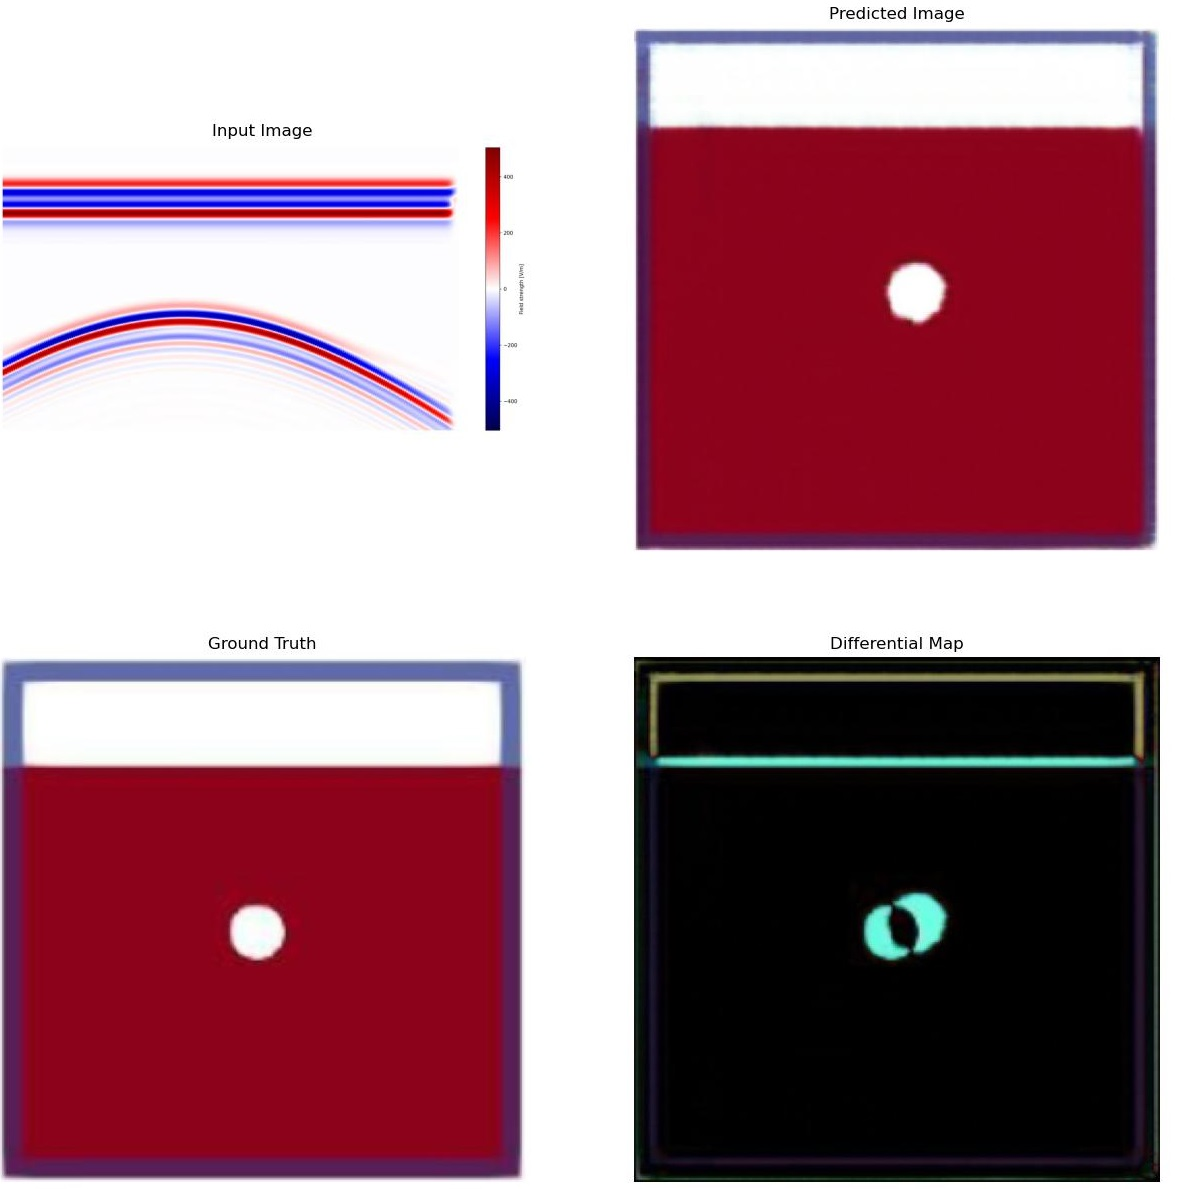
\includegraphics[scale=0.15]{gambar/diffMapLingkaran.jpg}
  \caption{Evaluasi Visual Data Variasi Bentuk Regular Lingkaran}
  \label{fig:diffmaplingkaran}
\end{figure}

Data ketiga dari variasi objek lingkaran memiliki nilai evaluasi matriks yang cukup buruk dari data lain dari variasi yang sama. 
Evaluasi visual dari data dapat dilihat dari gambar \ref{fig:diffmaplingkaran}. 
Pada gambar evaluasi visual dapat dilihat bahwa irisan dari objek sintesis dengan objek asli cukup sedikit sehingga memiliki area error yang cukup luas. 
Hal ini menunjukkan bahwa posisi benda belum sepenuhnya dapat dideteksi oleh model.

\begin{figure}[ht]
  \centering
  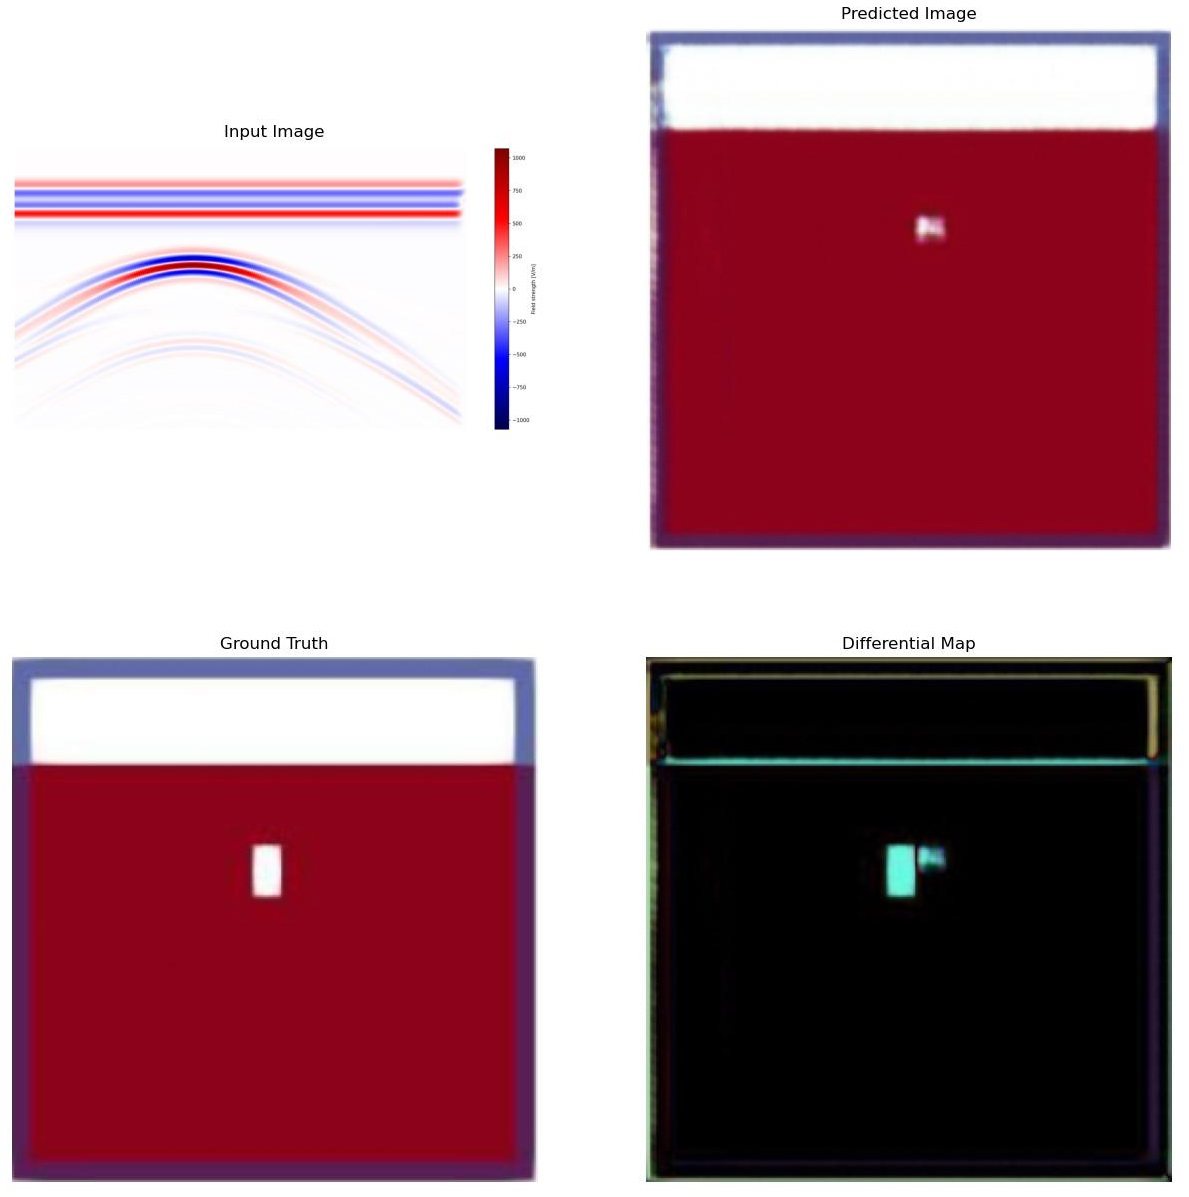
\includegraphics[scale=0.15]{gambar/diffMapSegi4.jpg}
  \caption{Evaluasi Visual Data Variasi Bentuk Regular Segi Empat}
  \label{fig:diffmapsegi4}
\end{figure}

Data kedua dari variasi objek segi empat memiliki nilai evaluasi matriks yang cukup baik dari data lain dari variasi yang sama. 
Evaluasi visual dari data dapat dilihat dari gambar \ref{fig:diffmapsegi4}. 
Pada gambar evaluasi visual dapat dilihat bahwa tidak ada irisan dari gambar sintesis dengan gambar asli, bahkan gambar sintesis hampir tidak memiliki bentuk. 
Hal ini menunjukkan bahwa model masih belum bisa mensintesis gambar dari objek regular berbentuk persegi, yang disebabkan oleh kurangnya data yang dipelajari ketika proses training model.

Pada variasi kompleksitas bentuk objek, terlihat untuk objek berbentuk sederhana memiliki rata-rata nilai evaluasi matriks yang lebih baik dari objek berbentuk kompleks. 
Perbedaan rata-rata evaluasi matriks terlihat cukup dekat di antara kedua variasi data.  
Nilai rata-rata SSIM data objek sederhana yang lebih kecil dari nilai rata-rata SSIM data objek kompleks. 
Namun, nilai rata-rata RMS dan MSE data objek sederhana lebih kecil dari nilai rata-rata RMS dan MSE data objek kompleks. 

\begin{figure}[ht]
  \centering
  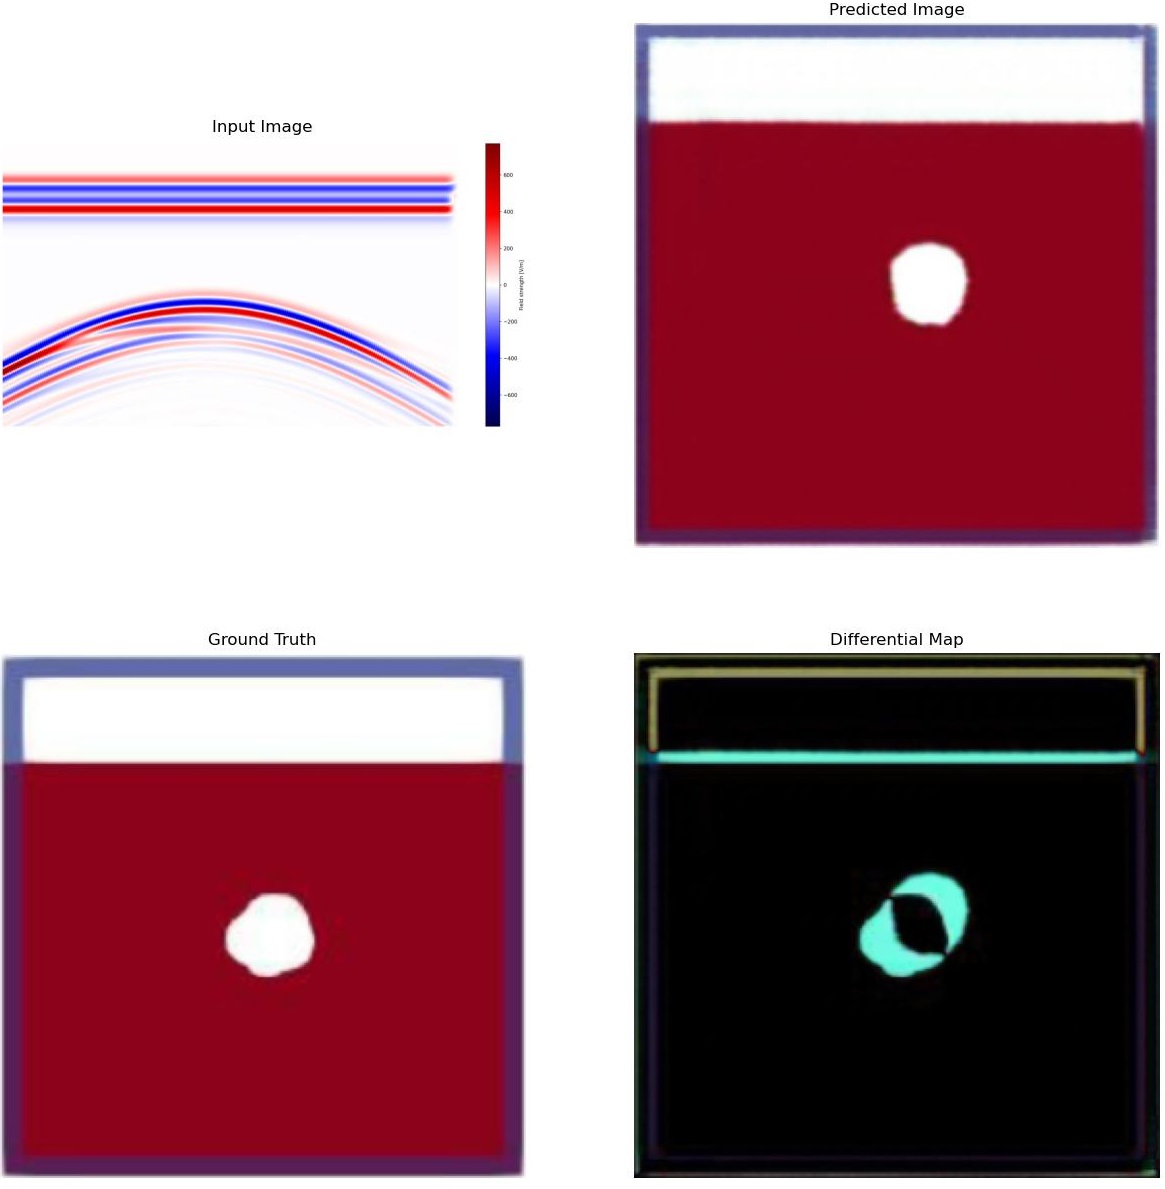
\includegraphics[scale=0.15]{gambar/diffMapSederhana.jpg}
  \caption{Evaluasi Visual Data Variasi Bentuk Sederhana}
  \label{fig:diffmapsederhana}
\end{figure}

Untuk variasi data dengan objek sederhana akan diambil data kedua karena memiliki nilai SSIM yang lebih buruk dari data lain. 
Evaluasi visual dari data dapat dilihat dari gambar \ref{fig:diffmapsederhana}.
Pada gambar evaluasi visual dapat dilihat bahwa irisan dari objek sintesis dengan objek asli cukup sedikit sehingga memiliki area error yang cukup luas. 
Hal ini menunjukkan bahwa posisi benda belum sepenuhnya dapat dideteksi oleh model.

\begin{figure}[ht]
  \centering
  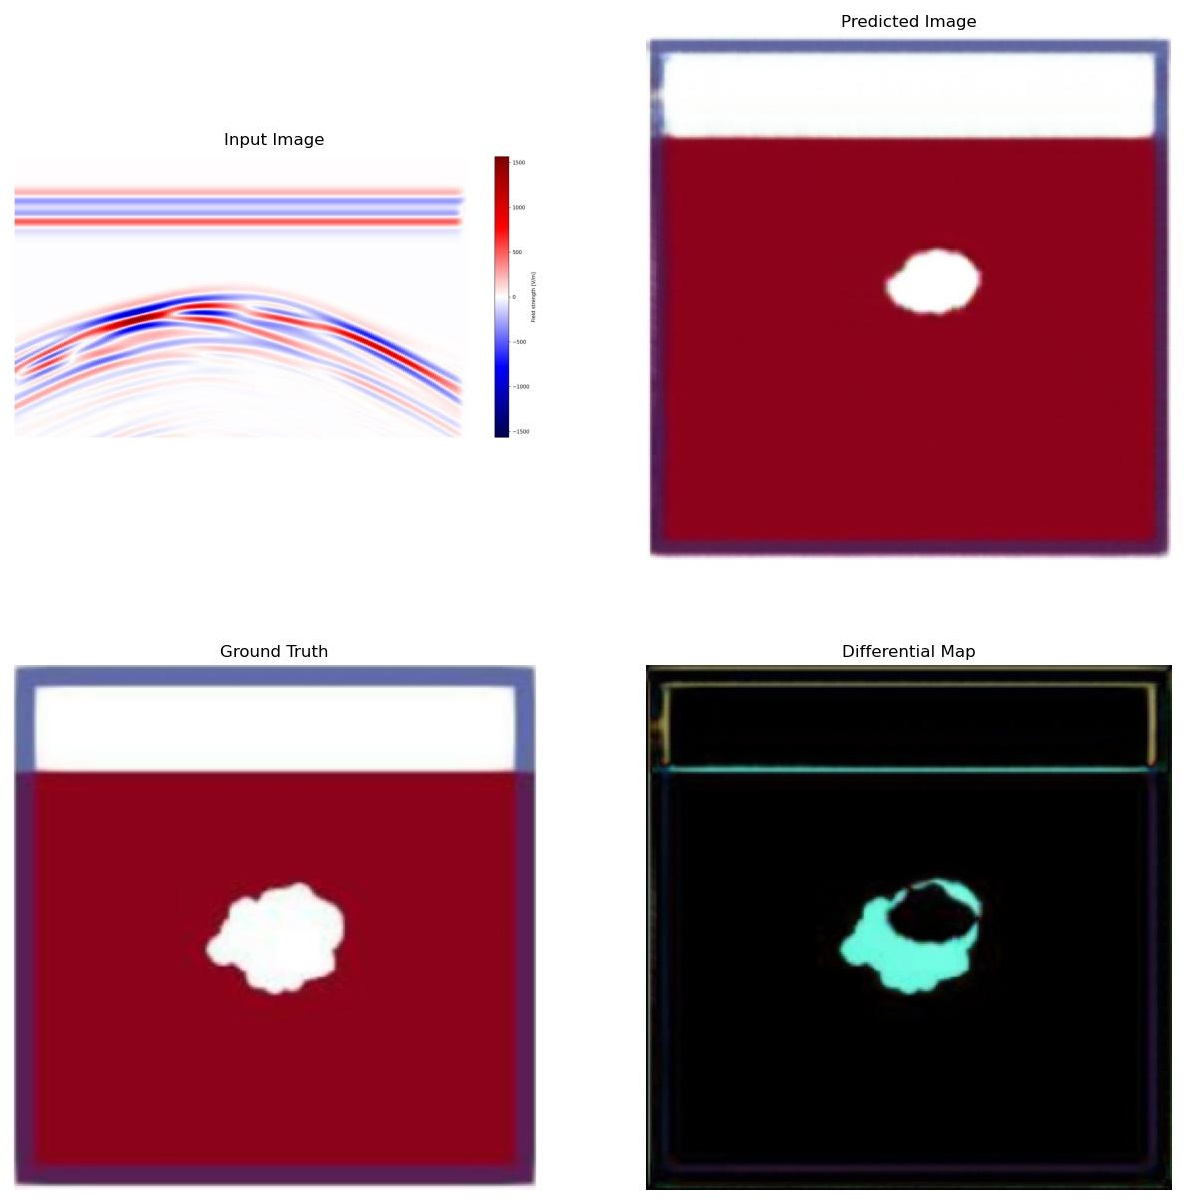
\includegraphics[scale=0.15]{gambar/diffMapKompleks.jpg}
  \caption{Evaluasi Visual Data Variasi Bentuk Kompleks}
  \label{fig:diffmapkompleks}
\end{figure}

Untuk variasi data dengan objek kompleks akan diambil data pertama karena memiliki nilai SSIM yang lebih baik dari data lain. 
Evaluasi visual dari data dapat dilihat dari gambar \ref{fig:diffmapkompleks}. 
Pada gambar evaluasi visual dapat dilihat bahwa irisan dari gambar sintesis dengan gambar asli merupakan gambar sintesis sepenuhnya. 
Hal ini menunjukkan bahwa model sudah bisa memprediksi posisi objek, namun masih belum bisa mensintesis ukuran objek dari objek berbentuk kompleks.

Pada variasi ukuran objek, terlihat untuk objek berukuran kecil memiliki rata-rata nilai evaluasi matriks yang lebih baik dari objek berukuran besar. 
Perbedaan rata-rata RMS dan MSE terlihat cukup jauh di antara kedua variasi data, sedangkan rata-rata SSIM terlihat cukup dekat. 
Namun, untuk beberapa data terdapat beberapa anomali, seperti data pertama dari variasi objek kecil dan data keempat dari objek besar. 

\begin{figure}[ht]
  \centering
  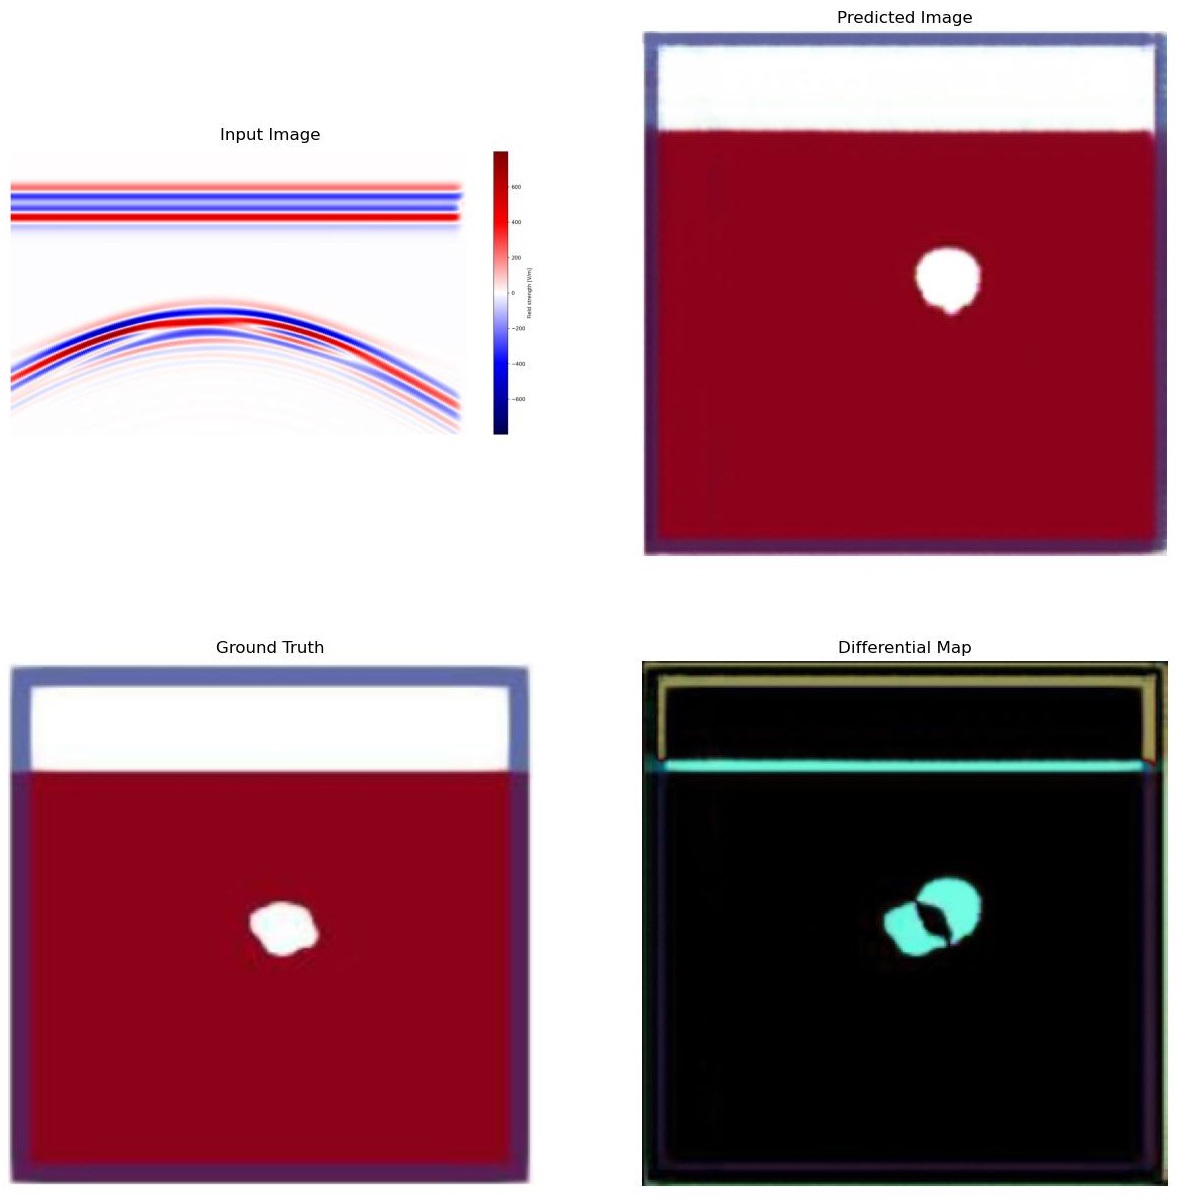
\includegraphics[scale=0.15]{gambar/diffMapKecil.jpg}
  \caption{Evaluasi Visual Data Variasi Ukuran Kecil}
  \label{fig:diffmapkecil}
\end{figure}

Data pertama dari variasi data dengan objek kecil memiliki nilai evaluasi matriks yang lebih buruk dari data lain. 
Evaluasi visual dari data dapat dilihat dari gambar \ref{fig:diffmapkecil}. 
Pada gambar evaluasi visual dapat dilihat bahwa irisan dari objek sintesis dengan objek asli cukup sedikit sehingga memiliki area error yang cukup luas. 
Hal ini menunjukkan bahwa posisi benda belum sepenuhnya dapat dideteksi oleh model.

\begin{figure}[ht]
  \centering
  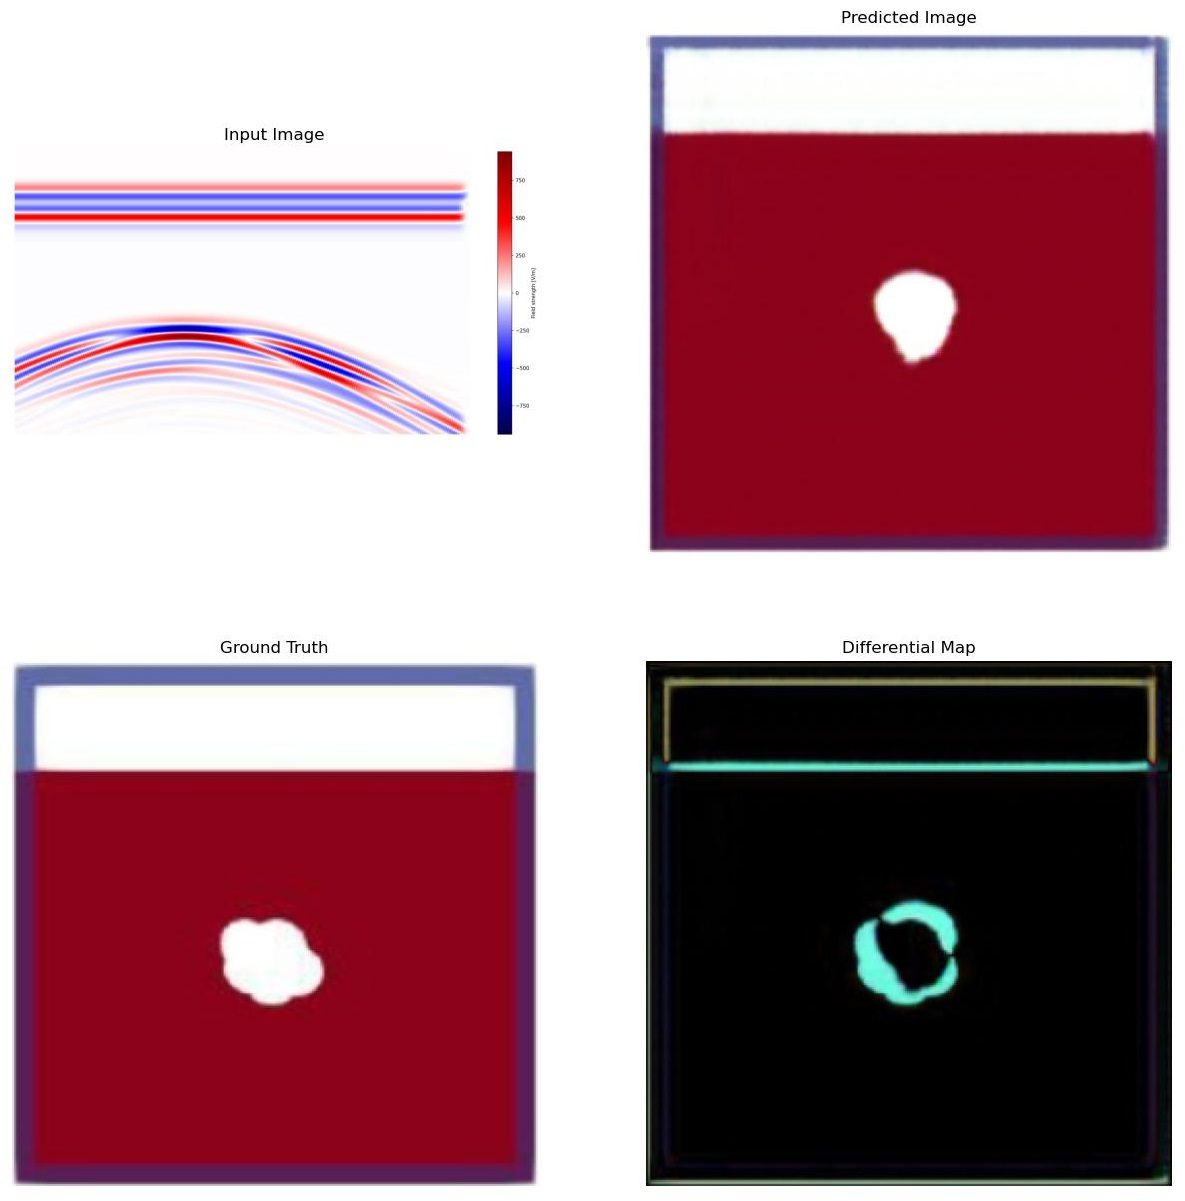
\includegraphics[scale=0.15]{gambar/diffMapBesar.jpg}
  \caption{Evaluasi Visual Data Variasi Ukuran Besar}
  \label{fig:diffmapbesar}
\end{figure}

Data keempat dari variasi data dengan objek besar karena memiliki nilai evaluasi matriks yang lebih baik dari data lain. 
Evaluasi visual dari data dapat dilihat dari gambar \ref{fig:diffmapbesar}. 
Pada gambar evaluasi visual dapat dilihat bahwa irisan dari objek sintesis dengan objek asli cukup luas sehingga memiliki area error yang cukup sedikit. 
Hal ini menunjukkan bahwa posisi beserta ukuran benda hampir dapat dideteksi oleh model. \\

Pada variasi posisi objek, terlihat untuk objek dengan posisi dekat dengan permukaan memiliki rata-rata nilai evaluasi matriks yang lebih baik dari objek dengan posisi jauh dengan permukaan. 
Perbedaan rata-rata evaluasi matriks terlihat cukup dekat di antara kedua variasi data, sedangkan rata-rata SSIM terlihat cukup jauh. 
Namun, untuk beberapa data terdapat beberapa anomali, seperti data ketiga dari variasi posisi objek dekat dari permukaan dan data ketiga dari variasi posisi objek jauh dari permukaan. 

\begin{figure}[ht]
  \centering
  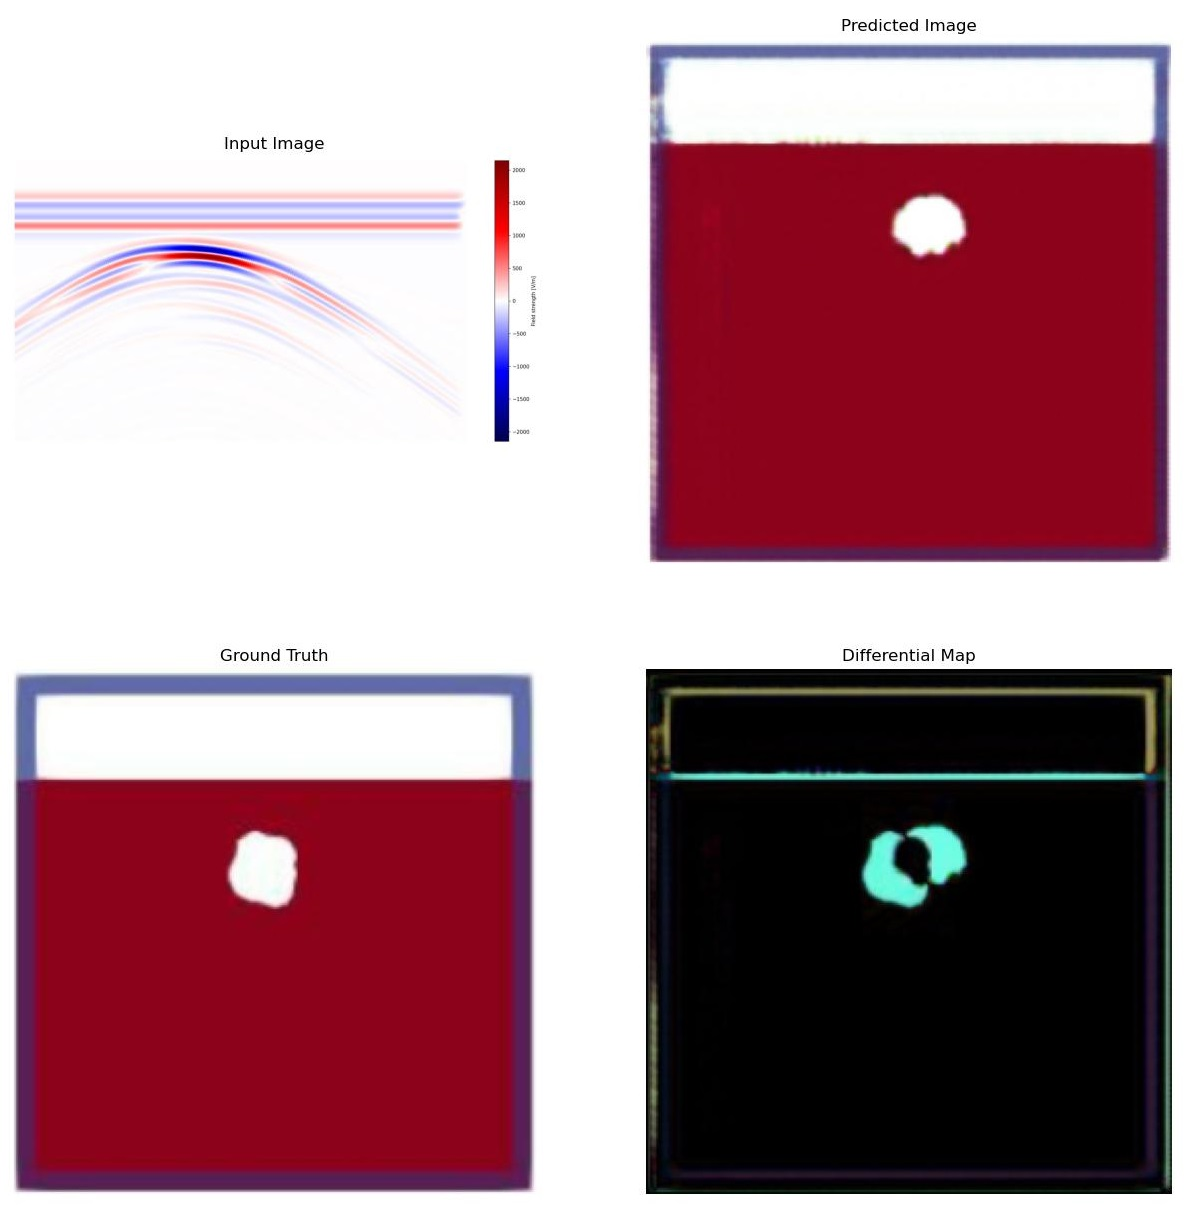
\includegraphics[scale=0.15]{gambar/diffMapDangkal.jpg}
  \caption{Evaluasi Visual Data Variasi Posisi Dekat dengan Permukaan}
  \label{fig:diffmapdangkal}
\end{figure}

Data ketiga dari variasi posisi objek dekat dengan permukaan memiliki nilai evaluasi matriks yang lebih buruk dari data lain. 
Evaluasi visual dari data dapat dilihat dari gambar \ref{fig:diffmapdangkal}. 
Pada gambar evaluasi visual dapat dilihat bahwa irisan dari objek sintesis dengan objek asli cukup sedikit sehingga memiliki area error yang cukup luas . 
Hal ini menunjukkan bahwa posisi beserta ukuran benda belum sepenuhnya dapat dideteksi oleh model.

\begin{figure}[ht]
  \centering
  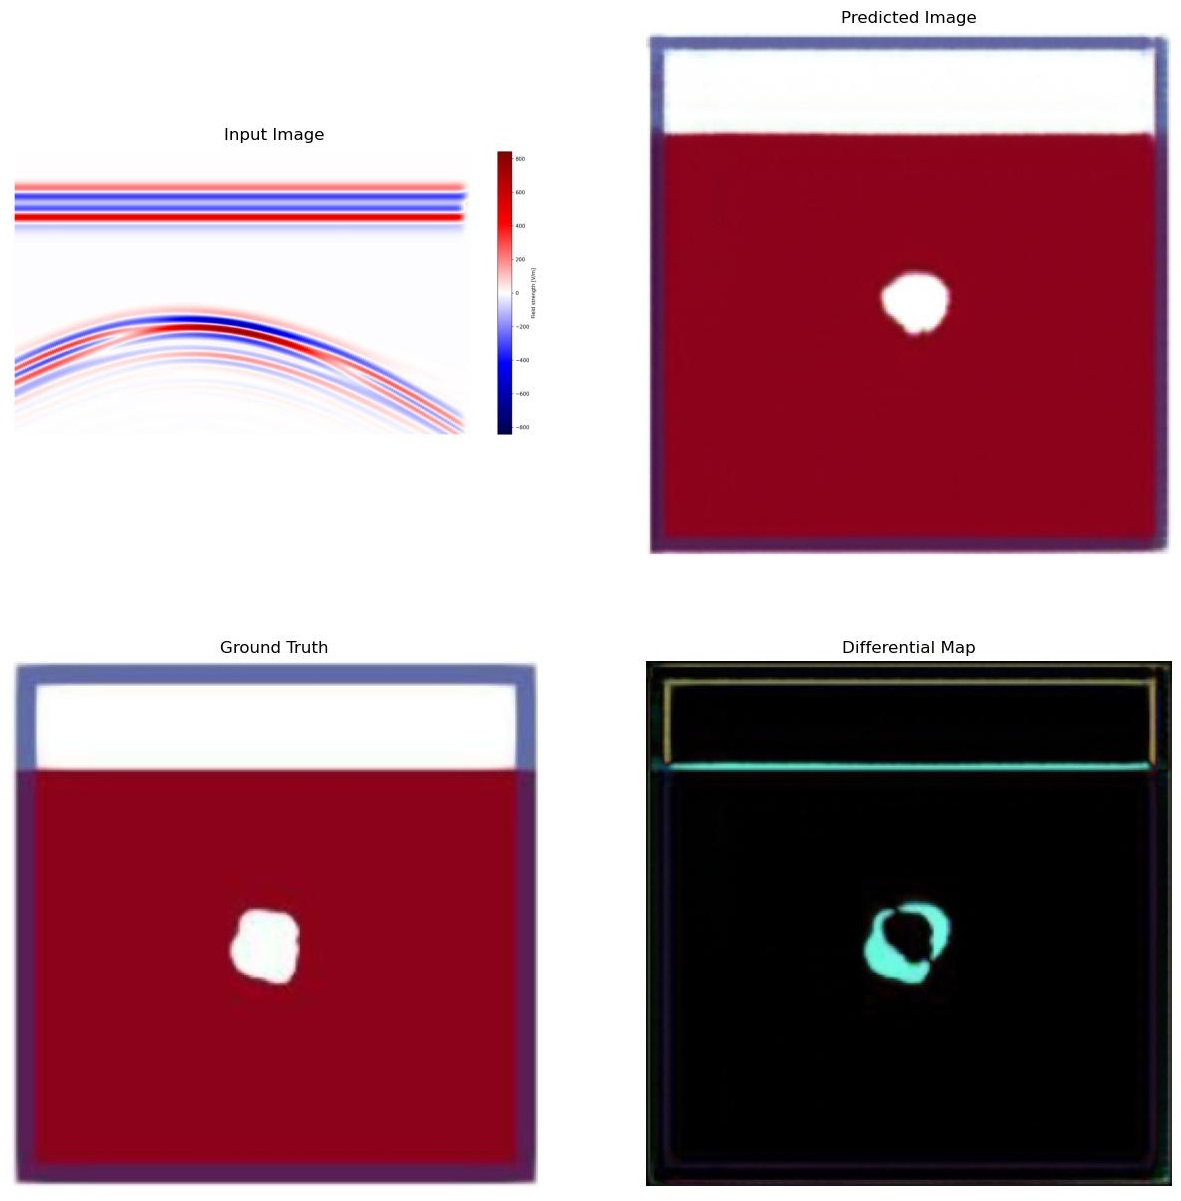
\includegraphics[scale=0.15]{gambar/diffMapDalam.jpg}
  \caption{Evaluasi Visual Data Variasi Posisi Jauh dengan Permukaan}
  \label{fig:diffmapdalam}
\end{figure}

Data ketiga dari variasi posisi objek jauh dengan permukaan memiliki nilai evaluasi matriks yang lebih buruk dari data lain. 
Evaluasi visual dari data dapat dilihat dari gambar \ref{fig:diffmapdalam}. 
Pada gambar evaluasi visual dapat dilihat bahwa irisan dari objek sintesis dengan objek asli cukup sedikit sehingga memiliki area error yang cukup luas. 
Hal ini menunjukkan bahwa posisi beserta ukuran benda belum sepenuhnya dapat dideteksi oleh model.  

Secara keseluruhan evaluasi matriks test data, diperoleh rata-rata RMS = 27.177, MSE = 1351.405, dan SSIM = 0.833. 
Tidak ada standar nilai RMS, MSE, dan SSIM yang bersifat universal atau mutlak untuk menentukan apakah suatu gambar dianggap baik atau buruk. 
Oleh karena itu, nilai rata-rata ini digunakan sebagai standar kemampuan model dalam menghasilkan data setiap variasinya.

Untuk variasi yang nilai rata-rata RMS dan MSE-nya lebih kecil dari nilai rata-rata RMS dan MSE total, dapat dikatakan intensitas piksel antara gambar yang disintesis dengan gambar asli hampir sama. 
Variasi tersebut diantaranya variasi bentuk regular lingkaran, bentuk regular segi empat, ukuran objek kecil, posisi objek dekat dari permukaan, dan posisi objek jauh dari permukaan. 
Sebaliknya, untuk variasi yang nilai rata-rata RMS dan MSE-nya lebih besar dari nilai rata-rata RMS dan MSE total, dapat dikatakan intensitas piksel antara gambar yang disintesis dengan gambar asli cukup jauh. 
Variasi tersebut diantaranya variasi bentuk objek sederhana, bentuk objek kompleks, dan ukuran objek besar.

Untuk variasi yang nilai rata-rata SSIM-nya lebih besar dari nilai rata-rata SSIM total, dapat dikatakan kesamaan struktural antara gambar yang disintesis dengan gambar asli hampir sama. 
Variasi tersebut diantaranya variasi bentuk regular lingkaran, bentuk regular segi empat, dan posisi objek jauh dari permukaan. 
Sebaliknya, untuk variasi yang nilai rata-rata SSIM-nya lebih kecil dari nilai rata-rata SSIM total, dapat dikatakan kesamaan struktural antara gambar yang disintesis dengan gambar asli cukup jauh. 
Variasi tersebut diantaranya variasi bentuk objek sederhana, bentuk objek kompleks, ukuran objek kecil, ukuran objek besar, dan posisi objek jauh dari permukaan.

\section{Kesimpulan dan Saran}

Hasil penelitian dari penggunaan model GAN untuk merekonstruksi sinyal B-scan GPR pada objek berbentuk irregular menunjukkan bahwa Model GAN mampu mempelajari pembuatan dari gambar input yang berupa B-scan GPR menjadi gambar struktur geometri bawah permukaan beton. 
Output model GAN mampu menunjukkan sedikit kesamaan posisi dan ukuran objek dengan objek pada ground truth.
Namun, bentuk dari objek dengan variasi bentuk yang lebih kompleks, lebih besar, atau berbentuk segi empat masih belum sesuai dengan ground truth yang diharapkan.

Untuk pengembangan lebih lanjut pada penelitian tugas akhir ini, penulis menyarankan untuk dapat memperbanyak data train untuk variasi bentuk dan ukuran benda guna memaksimalkan hasil prediksi gambar.
Jenis objek dan media perambatan baru untuk sinyal GPR hasil simulasi gprMax juga dapat ditambahkan. Penelitian lebih lanjut juga dapat dikembangkan untuk bentuk sinyal GPR lainnya, yaitu A-scan maupun C-scan.

\section{Lampiran}

Segala keperluan yang digunakan dalam pembuatan penelitian ini disimpan pada github yang dapat diakses melalui link : MehhTerserah/TA-072-19-0040 (github.com)

\section{Ucapan Terima Kasih}

Penulis J.P.S mengucapkan terima kasih kepada keluarga penulis yang membantu penulis secara spiritual dan material dalam penyusunan artikel ini, 
bapak Dr. Supeno Mardi Susiki Nugroho, ST., MT. selaku Kepala Departemen Teknik Komputer, Fakultas Teknologi Elektro dan Informatika Cerdas (FTEIC), Institut Teknologi Sepuluh Nopember, 
bapak Dion Hayu Fandiantoro, S.T., M.Eng. selaku dosen pembimbing I dan bapak Arief Kurniawan, S.T, M.T. selaku dosen pembimbing II yang selalu memberikan arahan selama mengerjakan penelitian tugas akhir ini, 
Bapak-ibu dosen pengajar Departemen Teknik Komputer, atas pengajaran, bimbingan, serta perhatian yang diberikan kepada penulis selama ini.

\section*{Referensi}

Please number citations consecutively within brackets \cite{b1}. The 
sentence punctuation follows the bracket \cite{b2}. Refer simply to the reference 
number, as in \cite{b3}---do not use ``Ref. \cite{b3}'' or ``reference \cite{b3}'' except at 
the beginning of a sentence: ``Reference \cite{b3} was the first $\ldots$''

Number footnotes separately in superscripts. Place the actual footnote at 
the bottom of the column in which it was cited. Do not put footnotes in the 
abstract or reference list. Use letters for table footnotes.

Unless there are six authors or more give all authors' names; do not use 
``et al.''. Papers that have not been published, even if they have been 
submitted for publication, should be cited as ``unpublished'' \cite{b4}. Papers 
that have been accepted for publication should be cited as ``in press'' \cite{b5}. 
Capitalize only the first word in a paper title, except for proper nouns and 
element symbols.

For papers published in translation journals, please give the English 
citation first, followed by the original foreign-language citation \cite{b6}.

\begin{thebibliography}{00}
\bibitem{a1} Neal, A. (2004). Ground-penetrating radar and its use in sedimentology: Principles, problems and progress. Earth-Science Reviews, 66(3), 261–330. https://doi.org/https://doi.org/10.1016/j.earscirev.2004.01.004
\bibitem{a2} PUPR, B. (2015). Diklat pemeliharaan jembatan ii : Modul 2 perbaikan kerusakan berdasarkan bahan. https:/ /simantu.pu.go.id/epel/edok/2d370 Modul 2 - Perbaikan Kerusakan Berdasarkan Bahan.pdf
\bibitem{a3} Gurel, L., and Oguz, U. (2000). Three-dimensional fdtd modeling of a ground-penetrating radar. IEEE Transactions on Geoscience and Remote Sensing, 38(4), 1513–1521. https://doi.org/10.1109/36.851951
\bibitem{a4} van den Bosch, I., Lambot, S., Huynen, I., Marc, A., and Druyts, P. (2006). Accurate and efficient modeling of monostatic gpr signal of dielectric targets buried in stratified media. Journal of Electromagnetic Waves and Applications, 20, 283–290. https : / / doi . org/ 10.1163/156939306775701704
\bibitem{a5} Liu, H., Xing, B., Wang, H., Cui, J., and Spencer, B. F. (2019). Simulation of ground penetrating radar on dispersive media by a finite element time domain algorithm. Journal of Applied Geophysics, 170, 103821. https: / / doi.org/ https: / / doi.org/10.1016/ j.jappgeo.2019.103821
\bibitem{a6} Irving, J., Knoll, M., and Knight, R. (2007). Improving crosshole radar velocity tomograms: A new approach to incorporating high-angle traveltime data. Geophysics, 72, J31–J41. https://doi.org/10.1190/1.2742813
\bibitem{a7} Liu, S., Lei, L., Fu, L., and Wu, J. (2014). Application of pre-stack reverse time migration based on fwi velocity estimation to ground penetrating radar data. Journal of Applied Geophysics, 1–7.
\bibitem{a8} Kruk, J., Liu, T., Mozaffari, A., Gueting, N., Klotzsche, A., Vereecken, H., Warren, C., and Giannopoulos, A. (2018). Gpr full-waveform inversion, recent developments, and future opportunities, 1–6. https://doi.org/10.1109/ICGPR.2018.8441667
\bibitem{a9} Ishitsuka, K., Iso, S., Onishi, K., and Matsuoka, T. (2018). Object detection in ground-penetrating radar images using a deep convolutional neural network and image set preparation by migration. International Journal of Geophysics, 2018, 1–8. https:/ /doi.org/10.1155/2018/9365184
\bibitem{a10} Ren, S., He, K., Girshick, R., and Sun, J. (2017). Faster r-cnn: Towards real-time object detection with region proposal networks. IEEE Transactions on Pattern Analysis and Machine Intelligence, 39(6), 1137–1149. https://doi.org/10.1109/TPAMI.2016.2577031
\bibitem{a11} Jiang, P., Gu, F., Tu, C., and Chen, B. (2018, May). Difnet: Semantic segmentation by diffusionnetworks.
\bibitem{a12} Goodfellow, I., Pouget-Abadie, J., Mirza, M., Xu, B.,Warde-Farley, D., Ozair, S., Courville, A., and Bengio, Y. (2014). Generative adversarial networks. Advances in Neural Information Processing Systems, 3. https://doi.org/10.1145/3422622
\bibitem{a13} Liu, B., Ren, Y., Liu, H., Xu, H., Wang, Z., Cohn, A., and Jiang, P. (2021). Gprinvnet: Deep learning-based ground-penetrating radar data inversion for tunnel linings. IEEE Transactions on Geoscience and Remote Sensing, PP, 1–21. https://doi.org/10.1109/TGRS. 2020.3046454
\bibitem{b1} Rice,W. B. D. (2019). Applying generative adversarial networks to intelligent subsurface imaging and identification. ArXiv, abs/1905.13321
\bibitem{b2} Shen, Z., Erdogmus, E., Morcous, G., Cheng, C., Shang, Z., McCabe, T., and Kodsy, A. (2020). Early detection of near-surface void defects in concrete pavement using drone based thermography and gpr methods.
\bibitem{b3} Isola, P., Zhu, J.-Y., Zhou, T., and Efros, A. (2017). Image-to-image translation with conditional adversarial networks, 5967–5976. https://doi.org/10.1109/CVPR.2017.632
\bibitem{c1} Ronneberger, O., Fischer, P., and Brox, T. (2015). U-net: Convolutional networks for biomedical image segmentation. LNCS, 9351, 234–241. https://doi.org/10.1007/978-3-319-24574-4 28
\end{thebibliography}
\vspace{12pt}
\color{red}
IEEE conference templates contain guidance text for composing and formatting conference papers. Please ensure that all template text is removed from your conference paper prior to submission to the conference. Failure to remove the template text from your paper may result in your paper not being published.

\end{document}
